\documentclass[11pt]{article}

\usepackage[letterpaper,margin=0.78in,headheight=15pt]{geometry}
\usepackage[T1]{fontenc}
\usepackage[utf8]{inputenc}
\usepackage{lmodern}
\usepackage{microtype}
\usepackage{amsmath,amssymb,mathtools}
\usepackage{booktabs,tabularx,array,longtable,multirow}
\usepackage{enumitem}
\usepackage{xcolor}
\usepackage{graphicx}
\usepackage{caption}
\usepackage{subcaption}
\usepackage{float}
\usepackage{pdflscape}
\usepackage{tikz}
\usetikzlibrary{arrows.meta,positioning,calc,fit,backgrounds,decorations.pathreplacing,shapes.geometric,shapes.multipart}
\usepackage[most]{tcolorbox}
\usepackage{listings}
\usepackage{fancyhdr}
\usepackage{titlesec}
\usepackage{hyperref}
\usepackage[nameinlink,noabbrev]{cleveref}
\usepackage{xurl}

\definecolor{ink}{HTML}{18222D}
\definecolor{slate}{HTML}{4D5B6A}
\definecolor{violet}{HTML}{6D5BD0}
\definecolor{violetdark}{HTML}{4E3DA8}
\definecolor{teal}{HTML}{0C7C86}
\definecolor{bluegray}{HTML}{EAF0F5}
\definecolor{lavender}{HTML}{F0EDFF}
\definecolor{mint}{HTML}{E9F7F4}
\definecolor{amber}{HTML}{A86500}
\definecolor{amberbg}{HTML}{FFF5DD}
\definecolor{redish}{HTML}{A43842}
\definecolor{redbg}{HTML}{FFF0F1}
\definecolor{greenish}{HTML}{277A55}
\definecolor{greenbg}{HTML}{EAF7F0}

\hypersetup{
  colorlinks=true,
  linkcolor=violetdark,
  citecolor=teal,
  urlcolor=teal,
  pdftitle={Native T-SQL Language Service Foundation: Design, Implementation, and Validation Review},
  pdfauthor={Prepared for Karl Burtram},
  pdfsubject={vscode-mssql PR 22860, native TypeScript SQL language service and SQL scripting foundation}
}

\pagestyle{fancy}
\fancyhf{}
\lhead{vscode-mssql Native T-SQL Language Service}
\rhead{Design, Implementation, and Validation Review}
\cfoot{\thepage}
\renewcommand{\headrulewidth}{0.4pt}

\titleformat{\section}{\Large\bfseries\color{ink}}{\thesection}{0.7em}{}
\titleformat{\subsection}{\large\bfseries\color{violetdark}}{\thesubsection}{0.65em}{}
\titleformat{\subsubsection}{\normalsize\bfseries\color{teal}}{\thesubsubsection}{0.55em}{}

\setlist[itemize]{topsep=3pt,itemsep=2pt,parsep=1pt,leftmargin=1.45em}
\setlist[enumerate]{topsep=3pt,itemsep=2pt,parsep=1pt,leftmargin=1.65em}
\setlength{\parindent}{0pt}
\setlength{\parskip}{5.5pt}
\setlength{\emergencystretch}{2em}
\raggedbottom

\newcommand{\code}[1]{\texttt{\detokenize{#1}}}
\newcommand{\impl}{\textcolor{greenish}{\textbf{Implemented}}}
\newcommand{\valid}{\textcolor{teal}{\textbf{Validated}}}
\newcommand{\future}{\textcolor{amber}{\textbf{Future contract}}}
\newcommand{\target}{\textcolor{violetdark}{\textbf{Target invariant}}}
\newcommand{\gap}{\textcolor{redish}{\textbf{Open finding}}}
\newcommand{\reported}{\textcolor{slate}{\textbf{Reported evidence}}}
\newcommand{\na}{\textcolor{slate}{--}}
\newcommand{\yes}{\textcolor{greenish}{\checkmark}}
\newcommand{\partialmark}{\textcolor{amber}{$\triangle$}}
\newcommand{\no}{\textcolor{redish}{$\times$}}

\newtcolorbox{takeawaybox}[1][]{
  enhanced,breakable,colback=lavender,colframe=violet,
  boxrule=0.8pt,arc=2mm,left=2.5mm,right=2.5mm,top=1.8mm,bottom=1.8mm,
  fonttitle=\bfseries,title={Key takeaway},#1
}
\newtcolorbox{statusbox}[1][]{
  enhanced,breakable,colback=bluegray,colframe=slate,
  boxrule=0.7pt,arc=2mm,left=2.5mm,right=2.5mm,top=1.8mm,bottom=1.8mm,
  fonttitle=\bfseries,title={Evidence status},#1
}
\newtcolorbox{designbox}[1][]{
  enhanced,breakable,colback=mint,colframe=teal,
  boxrule=0.7pt,arc=2mm,left=2.5mm,right=2.5mm,top=1.8mm,bottom=1.8mm,
  fonttitle=\bfseries,title={Design invariant},#1
}
\newtcolorbox{boundarybox}[1][]{
  enhanced,breakable,colback=amberbg,colframe=amber,
  boxrule=0.7pt,arc=2mm,left=2.5mm,right=2.5mm,top=1.8mm,bottom=1.8mm,
  fonttitle=\bfseries,title={Scope boundary},#1
}
\newtcolorbox{warningbox}[1][]{
  enhanced,breakable,colback=redbg,colframe=redish,
  boxrule=0.7pt,arc=2mm,left=2.5mm,right=2.5mm,top=1.8mm,bottom=1.8mm,
  fonttitle=\bfseries,title={Current limitation},#1
}
\newtcolorbox{reviewbox}[1][]{
  enhanced,breakable,colback=redbg,colframe=redish,
  boxrule=0.9pt,arc=2mm,left=2.7mm,right=2.7mm,top=2mm,bottom=2mm,
  fonttitle=\bfseries,title={Current-head review finding},#1
}
\newtcolorbox{evidencebox}[1][]{
  enhanced,breakable,colback=bluegray,colframe=violetdark,
  boxrule=0.7pt,arc=2mm,left=2.5mm,right=2.5mm,top=1.8mm,bottom=1.8mm,
  fonttitle=\bfseries,title={Evidence boundary},#1
}

\lstdefinestyle{code}{
  basicstyle=\ttfamily\small,
  backgroundcolor=\color{bluegray},
  frame=single,
  rulecolor=\color{slate!50},
  keywordstyle=\bfseries\color{violetdark},
  commentstyle=\itshape\color{slate},
  stringstyle=\color{teal},
  showstringspaces=false,
  breaklines=true,
  columns=fullflexible,
  xleftmargin=0.5em,
  xrightmargin=0.5em,
  aboveskip=6pt,
  belowskip=6pt
}
\lstset{style=code}

\tikzset{
  >=Latex,
  every node/.style={font=\small,text=ink},
  comp/.style={draw=slate!65,rounded corners=2.5pt,fill=bluegray,align=center,inner sep=4pt,minimum height=10mm},
  engine/.style={comp,fill=lavender,draw=violet!75},
  model/.style={comp,fill=mint,draw=teal!75},
  host/.style={comp,fill=greenbg,draw=greenish!70},
  gate/.style={comp,fill=amberbg,draw=amber!70},
  ext/.style={comp,fill=white,draw=slate!55,dashed},
  risk/.style={comp,fill=redbg,draw=redish!70},
  targetnode/.style={comp,fill=lavender,draw=violetdark!80,dashed},
  currentnode/.style={comp,fill=redbg,draw=redish!75},
  state/.style={draw=slate!60,rounded corners=7pt,fill=bluegray,minimum width=24mm,minimum height=9mm,align=center,inner sep=3pt},
  goodstate/.style={state,fill=greenbg,draw=greenish!70},
  arrow/.style={->,very thick,draw=ink!75},
  async/.style={->,thick,dashed,draw=violetdark!80},
  dataarr/.style={->,thick,draw=teal!85},
  failarr/.style={->,thick,dashed,draw=redish!80},
  note/.style={draw=slate!30,rounded corners=2pt,fill=white,align=left,inner sep=4pt,font=\footnotesize},
  labelbox/.style={font=\scriptsize,align=center,fill=white,inner sep=1.2pt},
  pill/.style={draw=slate!35,rounded corners=7pt,fill=white,inner xsep=5pt,inner ysep=2pt,font=\scriptsize\bfseries}
}

\begin{document}
\hypersetup{pageanchor=false}

\begin{titlepage}
\thispagestyle{empty}
\enlargethispage{0.28in}
\vspace*{0.22in}

{\color{violetdark}\rule{\textwidth}{2.2pt}}
\vspace{0.18in}

{\Huge\bfseries\color{ink} Native T-SQL Language Service\par}
\vspace{0.08in}
{\LARGE\bfseries\color{violetdark} Pure Analysis, Pinned Metadata, Feature Routing, and SQL Scripting\par}
\vspace{0.10in}
{\Large\color{slate} Design, implementation, and validation review\par}

\vspace{0.20in}
{\large For \href{https://github.com/microsoft/vscode-mssql/pull/22860}{vscode-mssql PR \#22860}\par}

\vspace{0.20in}
\begin{tcolorbox}[enhanced,colback=lavender,colframe=violet,boxrule=1pt,arc=2mm,left=4mm,right=4mm,top=2.6mm,bottom=2.6mm]
\textbf{Central question.} How can vscode-mssql replace remote, document-coupled language features with a deterministic TypeScript engine that remains useful on incomplete SQL, pins one immutable metadata generation per answer, distinguishes syntax truth from catalog-dependent claims, and refuses to turn uncertainty into false diagnostics or authoritative scripts?
\end{tcolorbox}

\vspace{0.09in}
\begin{tcolorbox}[enhanced,colback=amberbg,colframe=amber,boxrule=0.9pt,arc=2mm,left=4mm,right=4mm,top=2.4mm,bottom=2.4mm]
\textbf{Assessment at the reviewed head.} PR \#22860 establishes a coherent, source-only language and scripting foundation. Its dependency boundaries, pinned metadata seam, deterministic feature pipeline, stale-safe diagnostics scheduler, and strict scripting provenance are sound. Review commit \code{b66db2d8f} closes the original 26 threads and one immediate follow-up, including the eight reproduced ordinary-SQL trust defects. Commit \code{2bc5811e3} closes the later spaced alias-column-list residual and implements the full T-SQL positional rename semantics for derived and VALUES sources; commits \code{2c20cc170}/\code{2a54ec071} then close the final Copilot thread by guarding degenerate DML shapes (\code{DEFAULT VALUES} and explicit placeholders instead of invalid empty lists). Exact-head targeted validation passes 709 owned language/scripting tests plus seven observability tests (716/716); the preceding full sign-off also passed the 4,742-test broad MSSQL lane, SQL Projects, build, lint, formatting, hooks, and online packaging with a zero-byte VSIX delta. All 29 threads are resolved, every reported hosted lane is green at the snapshot, and the branch is mergeable; consumer activation remains gated independently on preview composition and integration proof.
\end{tcolorbox}

\vspace{0.14in}
\begin{tabular}{@{}ll@{}}
Prepared for: & Karl Burtram\\
Primary change: & \code{dev/karlb/query_05_language_service} at \code{2a54ec071}\\
Extraction base: & \code{95cf790e5}; 59 files, +26,468 / -0\\
Live PR base: & \code{53b707bbe} on \code{main}\\
Current \code{main}: & \code{c6d2baa442}; topic ahead 6 / behind 9\\
Metadata prerequisite: & merged PR \#22836 / shared metadata substrate\\
Focused corpus: & 709 owned / 716 exact-head targeted tests\\
Report snapshot: & 31 August 2026, America/Los\_Angeles\\
\end{tabular}

\vspace{0.11in}
{\small\color{slate}
This is an as-built, evidence-qualified report. Historical design notes explain intent; the pinned implementation, exact-head tests, live review state, Actions state, and package artifacts control where the documents and implementation differ.}

\end{titlepage}

\hypersetup{pageanchor=true}
\pagenumbering{roman}
\setcounter{tocdepth}{1}
\tableofcontents
\clearpage
\pagenumbering{arabic}

\section*{How to read this report}
\addcontentsline{toc}{section}{How to read this report}

The report keeps implementation, intended invariants, executable evidence, and future integration separate:

\begin{description}[leftmargin=2.15cm,style=nextline]
  \item[\impl] Present in the pinned PR head and traced to source.
  \item[\target] A behavior or safety contract the library is intended to preserve.
  \item[\valid] Exercised by a named test, build lane, package check, or observed repository state.
  \item[\gap] A live review finding or evidence gap that remains at report freeze.
  \item[\reported] A source-attributed measurement or probe not independently rerun while preparing this document.
  \item[\future] A consumer, bridge, activation path, or maturity step not shipped by this PR.
\end{description}

\begin{takeawaybox}
PR \#22860 is not a replacement language service that users can turn on. It is the independently reviewable library beneath such a replacement: public data contracts, a tolerant analysis pipeline, native features, a pinned metadata adapter, strict scripting, routing/scheduling policies, observability, and tests. A later PR must supply a gated consumer and VS Code adaptation before any product behavior changes.
\end{takeawaybox}

\begin{evidencebox}
The strongest evidence is deterministic unit behavior and source-boundary inspection. Local packaging proves the tree packages; GitHub's package comparison more directly proves that the new source contributes zero size to the shipped VSIX at this head. Neither proves live-catalog semantic equivalence across the full T-SQL grammar. That is a later preview-graduation gate.
\end{evidencebox}


\section{Review snapshot and evidence model}

\subsection{Pinned repository state}

The review separates three different baselines that are easy to blur together. The feature was authored on extraction base \code{95cf790e5}; the pull request currently identifies \code{53b707bbe} as its live base; and the repository's \code{main} branch has since advanced to \code{c6d2baa442}. The exact reviewed topic is six commits ahead of and nine commits behind current \code{main}. This does not invalidate the isolated source review, but a future consumer must begin from refreshed \code{main}; a maintainer may also choose to refresh this inert extraction before merge.

\begin{table}[H]
\centering
\small
\caption{Current-head repository and evidence snapshot.}
\label{tab:snapshot}
\begin{tabularx}{\textwidth}{@{}p{0.23\textwidth}p{0.24\textwidth}X@{}}
\toprule
\textbf{Dimension} & \textbf{Observed value} & \textbf{What it proves}\\
\midrule
PR head & \code{2a54ec071} & Exact source and targeted validation target reviewed in this report.\\
Extraction base & \code{95cf790e5cfe} & Metadata PR \#22836 is already present in the authored topic history.\\
Live PR base & \code{53b707bbed5d} & Base recorded by the active pull request.\\
Current \code{main} & \code{c6d2baa44247} & Nine mainline-only commits remain outside the isolated topic.\\
Change size & 59 files; +26,468 / -0 & A large but isolated source extraction, dominated by new language, scripting, and test files.\\
GitHub workflows & All reported lanes green at the snapshot; merge state \code{CLEAN} & Build/test, CodeQL, normalization, packaging, and platform launch lanes completed successfully at the final head.\\
Package comparison & Target/head both 85,347 KiB; 0 KiB delta & The source was not an input to the shipped extension bundle.\\
Coverage & 94.34331\% patch at the reported run; 1,041 changed lines uncovered & Broad execution, but not semantic completeness; coverage is supporting evidence rather than the trust boundary.\\
Review state & 29 resolved threads; zero unresolved & The original closeout, alias-list residual, and degenerate-DML guard all have source-attributed dispositions.\\
\bottomrule
\end{tabularx}
\end{table}

\subsection{Evidence ladder}

\begin{figure}[H]
\centering
\resizebox{0.97\textwidth}{!}{%
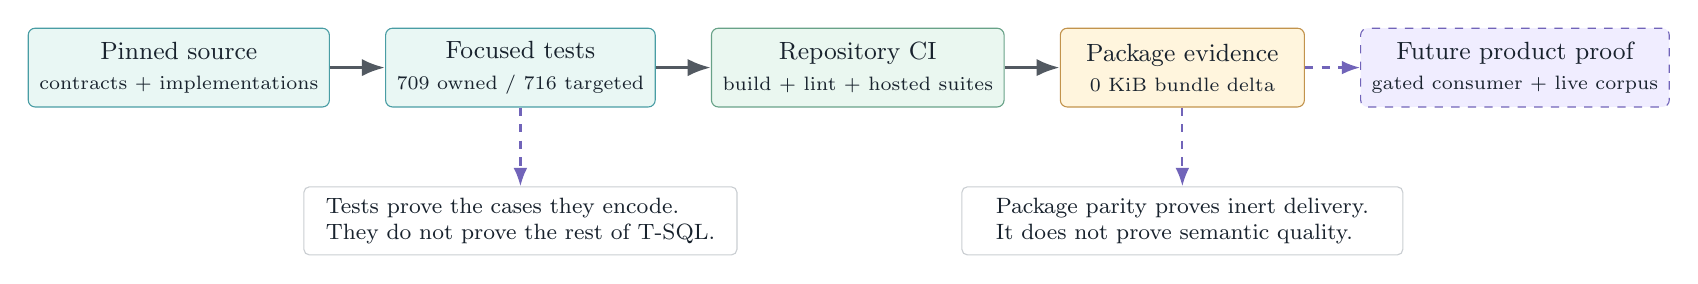
\begin{tikzpicture}[node distance=7mm and 7mm]
  \node[model,minimum width=31mm] (source) {Pinned source\\\scriptsize contracts + implementations};
  \node[model,minimum width=31mm,right=of source] (focused) {Focused tests\\\scriptsize 709 owned / 716 targeted};
  \node[host,minimum width=31mm,right=of focused] (ci) {Repository CI\\\scriptsize build + lint + hosted suites};
  \node[gate,minimum width=31mm,right=of ci] (package) {Package evidence\\\scriptsize 0 KiB bundle delta};
  \node[targetnode,minimum width=34mm,right=of package] (product) {Future product proof\\\scriptsize gated consumer + live corpus};

  \draw[arrow] (source)--(focused);
  \draw[arrow] (focused)--(ci);
  \draw[arrow] (ci)--(package);
  \draw[async] (package)--(product);

  \node[note,below=10mm of focused,minimum width=55mm] (semantic) {Tests prove the cases they encode.\\They do not prove the rest of T-SQL.};
  \node[note,below=10mm of package,minimum width=56mm] (scope) {Package parity proves inert delivery.\\It does not prove semantic quality.};
  \draw[async] (focused)--(semantic);
  \draw[async] (package)--(scope);
\end{tikzpicture}}
\caption{Evidence ladder. Each layer strengthens a different claim; green CI and zero package delta cannot substitute for a live semantic truth corpus.}
\label{fig:evidence-ladder}
\end{figure}

\begin{evidencebox}
The strongest current claims are architectural isolation, deterministic behavior on the focused corpus, package invisibility, and repair coverage for all current review findings. The weakest claim remains real-world semantic authority across the full T-SQL grammar. The external differential review improved the honesty corpus and found a residual whitespace variant that the final commit then repaired; that sequence shows why activation requires a broader live differential corpus rather than relying on aggregate coverage alone.
\end{evidencebox}

\subsection{Executive scorecard}

\begin{table}[H]
\centering
\small
\caption{Design objective versus current evidence.}
\label{tab:scorecard}
\begin{tabularx}{\textwidth}{@{}p{0.28\textwidth}cX@{}}
\toprule
\textbf{Objective} & \textbf{State} & \textbf{Assessment}\\
\midrule
Pure, consumer-neutral engine boundary & \yes & JSON-safe, VS Code-neutral contracts and linted import direction.\\
One metadata generation per answer & \yes & Every feature pins an immutable view; definition is the single sanctioned lazy read.\\
No metadata wait on keystroke paths & \yes & Interactive features read synchronously and may only request background hydration.\\
Honest diagnostic suppression & \yes & The original eight reproduced defects and the later spaced/newline alias-column-list variant are repaired and regression-tested.\\
Stale-result containment & \yes & Scheduled diagnostics stamp document version plus metadata generation and abort stale publication.\\
Per-feature fallback containment & \partialmark & Throw/rejection circuits work; a timer cannot preempt synchronous extension-host CPU work.\\
Strict scripting provenance & \yes & Freshness/refusal/offline provenance and pathological comment sanitization are explicit and regression-tested.\\
Production metadata-adapter confidence & \partialmark & A real builder/snapshot/provider-to-engine test now exists; broader live-server and generation-drift coverage remains preview work.\\
Private-preview invisibility & \yes & No activation, provider registration, command, setting, or bundle input lands in this PR.\\
Current-main merge readiness & \partialmark & The branch is mergeable with zero unresolved threads and green hosted lanes; human re-approval of the post-sign-off fix commits is pending and the topic is nine mainline commits behind.\\
\bottomrule
\end{tabularx}
\end{table}

\section{Executive summary}

\subsection{What the PR establishes}

The change adds 37 production files under \path{src/sqlLanguage}, six under \path{src/sqlScripting}, fifteen focused unit files, and one observability classification edit. The architecture has four load-bearing properties:

\begin{enumerate}
  \item \textbf{Pure request contracts and analysis.} Positions are zero-based UTF-16; payloads are JSON-safe; the core has no VS Code document or provider types.
  \item \textbf{One truth generation per request.} Language work pins one immutable metadata view and reads readiness, environment, names, columns, parameters, keys, and definitions through that generation-stable seam.
  \item \textbf{Honest partial behavior.} Absence and unavailability are different. The engine suppresses metadata-dependent claims, returns incomplete completion where appropriate, and preserves lexical/structural diagnostics when catalog validation is unavailable.
  \item \textbf{Source-only private-preview boundary.} There is no package contribution, command, setting, activation event, controller, provider registration, Query Studio bridge, or AI consumer. Existing users cannot reach the code from this PR.
\end{enumerate}

\subsection{What the PR does not establish}

It does not claim full T-SQL parsing, ScriptDOM equivalence, semantic-token or document-highlight support, live runtime integration, a production latency service-level objective, or a user-visible migration from the current SQL Tools Service language providers. The router includes a lazy bridge seam, but the bridge itself and the host composition that chooses it are deferred.

\begin{boundarybox}[title={Private-preview meaning in this PR}]
No dedicated setting is added because there is no activated feature to gate. That is safer than a dead setting that suggests usable behavior. The first integration PR must require the umbrella experimental/private-preview flag \emph{and} a dedicated feature-area flag, default both off, hide all contributed UI, and register runtime consumers only when the effective gate is true at activation.
\end{boundarybox}


\subsection{The claim hierarchy}

The implementation is best understood as a ladder of increasingly expensive claims. Each higher level depends on every lower level plus additional authority. When a lower level is uncertain, the engine should retain lower-level usefulness and remove the unsupported higher-level claim.

\begin{figure}[H]
\centering
\resizebox{0.93\textwidth}{!}{%
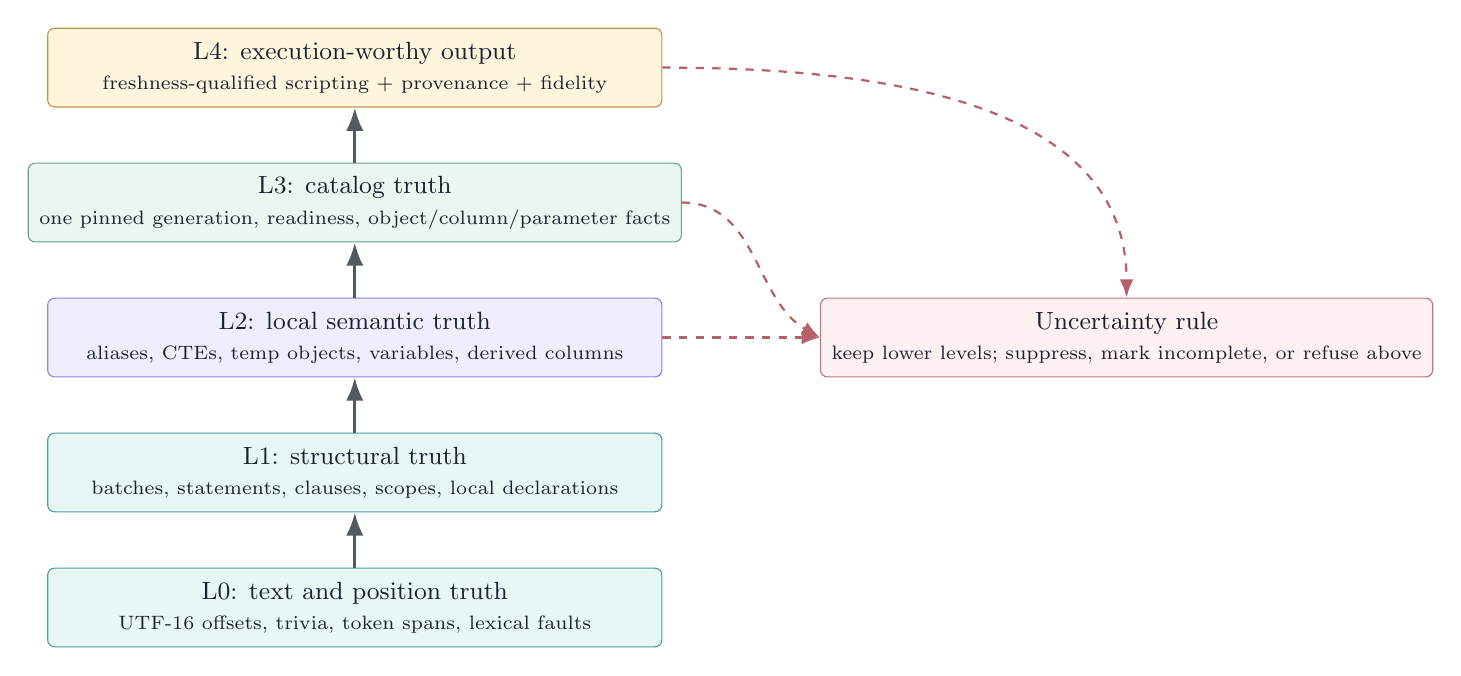
\begin{tikzpicture}[node distance=7mm]
  \node[model,minimum width=78mm] (l0) {L0: text and position truth\\\scriptsize UTF-16 offsets, trivia, token spans, lexical faults};
  \node[model,minimum width=78mm,above=of l0] (l1) {L1: structural truth\\\scriptsize batches, statements, clauses, scopes, local declarations};
  \node[engine,minimum width=78mm,above=of l1] (l2) {L2: local semantic truth\\\scriptsize aliases, CTEs, temp objects, variables, derived columns};
  \node[host,minimum width=78mm,above=of l2] (l3) {L3: catalog truth\\\scriptsize one pinned generation, readiness, object/column/parameter facts};
  \node[gate,minimum width=78mm,above=of l3] (l4) {L4: execution-worthy output\\\scriptsize freshness-qualified scripting + provenance + fidelity};

  \draw[arrow] (l0)--(l1);
  \draw[arrow] (l1)--(l2);
  \draw[arrow] (l2)--(l3);
  \draw[arrow] (l3)--(l4);

  \node[risk,right=20mm of l2,minimum width=48mm] (uncertain) {Uncertainty rule\\\scriptsize keep lower levels; suppress, mark incomplete, or refuse above};
  \draw[failarr] (l4.east) to[out=0,in=90] (uncertain.north);
  \draw[failarr] (l3.east) to[out=0,in=150] (uncertain.west);
  \draw[failarr] (l2.east)--(uncertain.west);
\end{tikzpicture}}
\caption{Claim hierarchy. The engine is useful before it is omniscient: uncertainty removes authority rather than fabricating certainty.}
\label{fig:claim-hierarchy}
\end{figure}

\begin{designbox}[title={The central safety invariant}]
A missing token may reduce structural confidence; a missing metadata section may reduce catalog confidence; an unvalidated snapshot may block scripting. None of those conditions should erase facts from a lower tier that remain independently true. This is why lexical diagnostics can continue while binder diagnostics are suppressed, and why keywords/local symbols can remain available while catalog completion is incomplete.
\end{designbox}

\section{Placement in the refactor train}

PR \#22860 is extraction PR05. The accepted refactor layers beneath it are already in the authored base: core observability, SQL Data Plane and STS2 transport, and the shared metadata substrate from PR \#22836. This PR adds the pure language/scripting library and the production metadata adapter, but deliberately stops before any VS Code or Query Studio consumer registration.

\begin{figure}[H]
\centering
\resizebox{0.96\textwidth}{!}{%
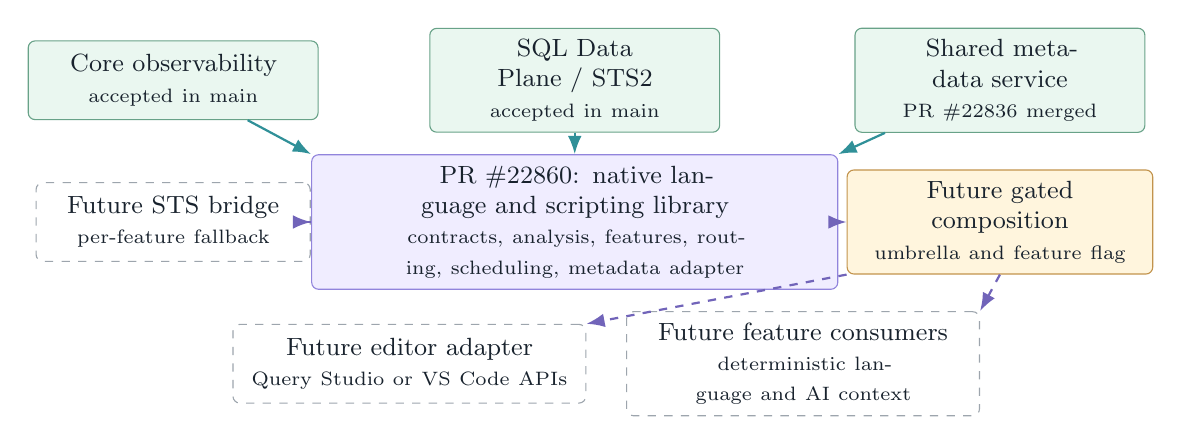
\begin{tikzpicture}[x=1cm,y=1cm]
  \node[host,text width=34mm] (obs) at (0.0,3.6) {Core observability\\{\scriptsize accepted in main}};
  \node[host,text width=34mm] (dp) at (5.1,3.6) {SQL Data Plane / STS2\\{\scriptsize accepted in main}};
  \node[host,text width=34mm] (metadata) at (10.5,3.6) {Shared metadata service\\{\scriptsize PR \#22836 merged}};

  \node[ext,text width=32mm] (bridge) at (0.0,1.8) {Future STS bridge\\{\scriptsize per-feature fallback}};
  \node[engine,text width=64mm] (lang) at (5.1,1.8) {PR \#22860: native language and scripting library\\{\scriptsize contracts, analysis, features, routing, scheduling, metadata adapter}};
  \node[gate,text width=36mm] (composition) at (10.5,1.8) {Future gated composition\\{\scriptsize umbrella and feature flag}};

  \node[ext,text width=42mm] (editor) at (3.0,0.0) {Future editor adapter\\{\scriptsize Query Studio or VS Code APIs}};
  \node[ext,text width=42mm] (consumer) at (8.0,0.0) {Future feature consumers\\{\scriptsize deterministic language and AI context}};

  \draw[dataarr] (obs)--(lang.north west);
  \draw[dataarr] (dp)--(lang.north);
  \draw[dataarr] (metadata)--(lang.north east);
  \draw[async] (bridge)--(lang);
  \draw[async] (lang)--(composition);
  \draw[async] (composition.south west)--(editor.north east);
  \draw[async] (composition.south)--(consumer.north east);
\end{tikzpicture}}
\caption{Refactor placement. Solid lower layers and the violet PR05 library exist; dashed consumer and fallback paths are intentionally absent from this pull request.}
\label{fig:placement}
\end{figure}

The package bot reports the MSSQL VSIX as 85,347 KiB on both target and PR branches, and the other packaged extensions also show zero delta. That is stronger scope evidence than merely observing that no command or setting was added: the build graph itself does not include the new source at this head.

\begin{boundarybox}[title={Branch-drift note}]
The PR was authored from extraction base \code{95cf790e5}; the active PR now names \code{53b707bbe} as its base, while current \code{main} is \code{c6d2baa442}. The nine-mainline-commit gap touches integration surfaces such as \path{mainController.ts}, \path{sqlDocumentService.ts}, package metadata, and general extension infrastructure. The language source remains isolated and preceding-head packaging is green; final-head packaging is rerunning. Every later consumer must start from refreshed \code{main} and rerun the integration assertions.
\end{boundarybox}

\section{Public contracts and dependency boundaries}

\subsection{Consumer-neutral API}

\path{sqlLanguage/api.ts} defines JSON-safe request and response data for completion, hover, signature help, diagnostics, definition, folding, document symbols, highlights, and semantic tokens. Point requests carry the full document text, a version, and a zero-based UTF-16 position; diagnostics/structure requests carry text and version. The contract deliberately carries no VS Code document, URI, cancellation token, metadata object, or STS DTO. A future host owns document identity, routing, cancellation, and translation to editor-native result types.

The v1 request shape sends the full document text on each call. That is a simple and highly testable extraction boundary, not a commitment to permanent full-text transport. A later Query Studio or VS Code adapter can add incremental synchronization or per-document engine instances without changing the pure feature algorithms.

The same file defines feature maturity and a capability table. The shipped native capability table marks completion, hover, signature, diagnostics, definition, folding, and document symbols as preview; highlights and semantic tokens remain off. Having types for a feature is therefore not the same as advertising an implementation.

\begin{table}[H]
\centering
\small
\caption{Public request-shape boundary.}
\label{tab:request-shapes}
\begin{tabularx}{\textwidth}{@{}p{0.22\textwidth}p{0.30\textwidth}X@{}}
\toprule
\textbf{Request family} & \textbf{Carries} & \textbf{Intentionally owned by the future host}\\
\midrule
Point features & Full text, version, UTF-16 line/character; completion also carries trigger kind/character & URI/document identity, connection binding, cancellation, VS Code/Monaco result adaptation.\\
Diagnostics/structure & Full text, version; diagnostics may carry a host-derived metadata freshness verdict & Debounce, scheduling, publication, editor marker ownership, current metadata stamp.\\
Definition/scripting & Point request plus target resolution; scripting request plus provenance/fidelity contracts & Virtual document storage, reveal behavior, strict lease policy, user-facing refusal UX.\\
\bottomrule
\end{tabularx}
\end{table}

\begin{table}[H]
\centering
\small
\caption{Native feature surface at the pinned head.}
\label{tab:features}
\begin{tabularx}{\textwidth}{@{}p{0.19\textwidth}p{0.17\textwidth}X@{}}
\toprule
\textbf{Feature} & \textbf{Capability} & \textbf{As-built behavior}\\
\midrule
Completion & Preview & Context/expectation-gated candidates, deterministic rank, partial-readiness honesty, lazy hydration kick.\\
Hover & Preview & Local, overlay, catalog, system, routine, built-in, and description facts when their readiness tier permits.\\
Signature help & Preview & Built-ins, catalog functions/procedures, nested calls, and \code{EXEC} argument tracking.\\
Diagnostics & Preview & T1 lexical/structural errors plus freshness-gated T2 208/207/209 binder warnings.\\
Definition & Preview & In-document local targets or virtual scripted catalog definitions with anchors and fidelity.\\
Folding & Preview & Batch, statement, comment, and region ranges.\\
Document symbols & Preview & Batch/statement structure and simple create/alter object declarations.\\
Highlights & Off & Interface reserved; native engine returns no result.\\
Semantic tokens & Off & Interface reserved; native engine returns no result.\\
\bottomrule
\end{tabularx}
\end{table}

\subsection{Purity and import direction}

Core analysis, feature computation, static data, provider interfaces, and scripting emitters are library code. Concrete host concerns live under \path{host}: metadata freshness, diagnostic journaling, timeout/yield behavior, and routing. The one sanctioned bridge from language metadata to the product catalog model is \path{provider/catalogProvider.ts}.

\begin{designbox}
Interactive feature code consumes a synchronous \code{IPinnedMetadataView}; it does not hold a mutable store, lease, network client, VS Code document, or STS service. Definition text is the one deliberate async lookup on the pinned view, and strict scripting asks the host to establish freshness before it creates the engine.
\end{designbox}

\section{Document analysis pipeline}

\subsection{From text to reusable structure}

The native engine analyzes one immutable text snapshot, then reuses structural work across feature calls. Review commit \code{b66db2d8f} strengthens both analysis and diagnostics memoization to require exact text identity in addition to version/length context. Same-version, same-length replacement text can no longer reuse the wrong analysis, while ordinary repeat requests still share immutable structural work.

The stages are deliberately tolerant:

\begin{enumerate}
  \item \textbf{Text snapshot} maps offsets to zero-based UTF-16 line/character positions and back, including ordinary LF/CRLF and mixed input.
  \item \textbf{Lexer} recognizes T-SQL words, identifiers, punctuation, comments, strings, variables, SQLCMD-sensitive regions, Unicode horizontal whitespace, and \code{GO} / \code{GO n} line semantics. Review repairs pin non-breaking-space classification and a construct opener at exact EOF.
  \item \textbf{Segmenter} partitions batches and statements while respecting module bodies and rule-sensitive constructs.
  \item \textbf{Sketch parser} extracts the structure features need: query scopes, sources, CTEs, select items, declarations, \code{EXEC}, DML targets, and table declarations. It remains total on incomplete editor text.
  \item \textbf{Overlay} models script-local state such as temporary tables, declared table variables, scripted tables, and batch-scoped variables.
  \item \textbf{Binder and cursor expectation} combine local structure, the effective database, and one pinned metadata view for a particular feature request.
\end{enumerate}

\begin{figure}[H]
\centering
\resizebox{0.98\textwidth}{!}{%
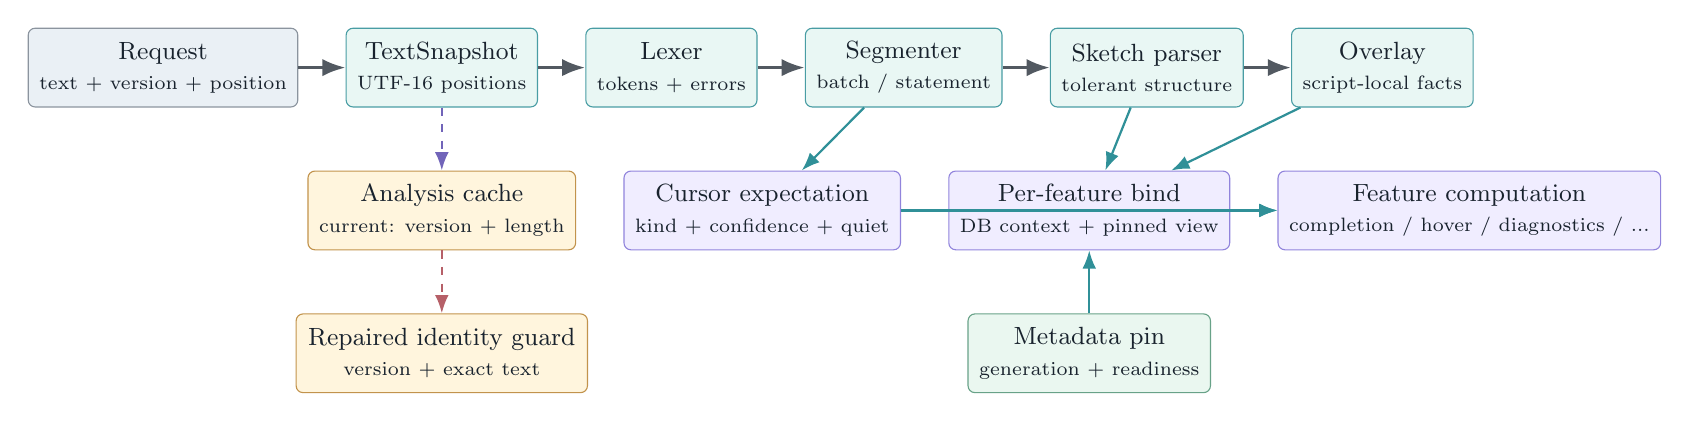
\begin{tikzpicture}[node distance=8mm and 6mm]
  \node[comp,minimum width=25mm] (request) {Request\\\scriptsize text + version + position};
  \node[model,minimum width=23mm,right=of request] (snapshot) {TextSnapshot\\\scriptsize UTF-16 positions};
  \node[model,minimum width=19mm,right=of snapshot] (lex) {Lexer\\\scriptsize tokens + errors};
  \node[model,minimum width=23mm,right=of lex] (segment) {Segmenter\\\scriptsize batch / statement};
  \node[model,minimum width=24mm,right=of segment] (sketch) {Sketch parser\\\scriptsize tolerant structure};
  \node[model,minimum width=23mm,right=of sketch] (overlay) {Overlay\\\scriptsize script-local facts};

  \node[gate,below=of snapshot,minimum width=27mm] (cache) {Analysis cache\\\scriptsize current: version + length};
  \node[engine,right=of cache,minimum width=27mm] (expect) {Cursor expectation\\\scriptsize kind + confidence + quiet};
  \node[engine,right=of expect,minimum width=29mm] (bind) {Per-feature bind\\\scriptsize DB context + pinned view};
  \node[engine,right=of bind,minimum width=34mm] (features) {Feature computation\\\scriptsize completion / hover / diagnostics / ...};
  \node[host,below=of bind,minimum width=30mm] (pin) {Metadata pin\\\scriptsize generation + readiness};

  \draw[arrow] (request)--(snapshot);
  \draw[arrow] (snapshot)--(lex);
  \draw[arrow] (lex)--(segment);
  \draw[arrow] (segment)--(sketch);
  \draw[arrow] (sketch)--(overlay);
  \draw[dataarr] (segment)--(expect);
  \draw[dataarr] (sketch)--(bind);
  \draw[dataarr] (overlay)--(bind);
  \draw[dataarr] (expect)--(features);
  \draw[dataarr] (bind)--(features);
  \draw[async] (snapshot)--(cache);
  \draw[dataarr] (pin)--(bind);
  \node[gate,below=8mm of cache,minimum width=37mm] (cacheRisk) {Repaired identity guard\\\scriptsize version + exact text};
  \draw[failarr] (cache)--(cacheRisk);
\end{tikzpicture}}
\caption{As-built analysis pipeline. Structural analysis is reused, metadata is pinned per request, and binding never mixes generations. The red review boundary is the analysis memo key: target identity should include document or content identity, not only version and length.}
\label{fig:pipeline}
\end{figure}

\subsection{One request, one pin, one answer}

\begin{figure}[H]
\centering
\resizebox{0.95\textwidth}{!}{%
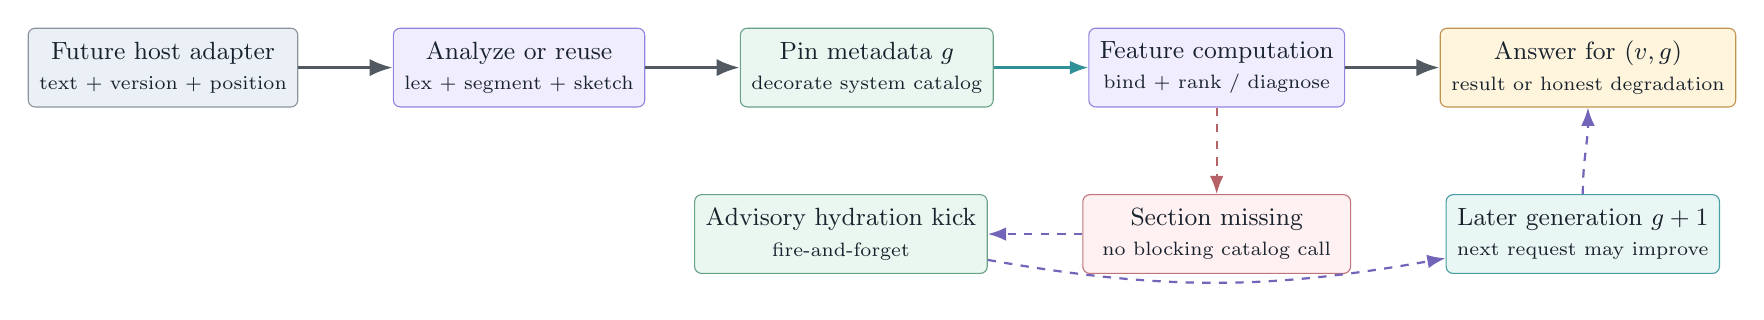
\begin{tikzpicture}[node distance=7mm and 12mm]
  \node[comp,minimum width=30mm] (host) {Future host adapter\\\scriptsize text + version + position};
  \node[engine,minimum width=29mm,right=of host] (analysis) {Analyze or reuse\\\scriptsize lex + segment + sketch};
  \node[host,minimum width=29mm,right=of analysis] (pin) {Pin metadata $g$\\\scriptsize decorate system catalog};
  \node[engine,minimum width=30mm,right=of pin] (feature) {Feature computation\\\scriptsize bind + rank / diagnose};
  \node[gate,minimum width=31mm,right=of feature] (answer) {Answer for $(v,g)$\\\scriptsize result or honest degradation};

  \node[risk,below=11mm of feature,minimum width=34mm] (missing) {Section missing\\\scriptsize no blocking catalog call};
  \node[host,left=of missing,minimum width=32mm] (kick) {Advisory hydration kick\\\scriptsize fire-and-forget};
  \node[model,right=of missing,minimum width=32mm] (next) {Later generation $g+1$\\\scriptsize next request may improve};

  \draw[arrow] (host)--(analysis);
  \draw[arrow] (analysis)--(pin);
  \draw[dataarr] (pin)--(feature);
  \draw[arrow] (feature)--(answer);
  \draw[failarr] (feature)--(missing);
  \draw[async] (missing)--(kick);
  \draw[async] (kick) to[out=-10,in=190] (next);
  \draw[async] (next) to[out=90,in=-90] (answer);
\end{tikzpicture}}
\caption{Interactive request lifecycle. A response is stamped by document version and one metadata generation; missing data can improve a later request but cannot mutate the answer already being produced.}
\label{fig:request-lifecycle}
\end{figure}


\subsection{Why a sketch instead of a full AST}

Editor input is commonly unfinished. A full grammar can make a single missing token collapse useful context; an unbounded hand-written parser can accidentally become a second compiler. The sketch deliberately extracts only what current features consume and records uncertainty. The cursor-expectation layer improves completion category selection and suppresses suggestions in declarations, data-type positions, comments, strings, and other quiet contexts, but it is not the richer parser-v2/AST envisioned by later design notes.

\begin{warningbox}[title={Semantic ceiling}]
The tolerant pipeline is broad, not complete. Dynamic SQL, unusual procedural forms, deeply dialect-specific syntax, and ambiguous recovery can exceed the sketch. The correct failure mode is suppression, incomplete results, or fallback--never a confident catalog error manufactured from an untrusted parse.
\end{warningbox}

\section{Metadata contract and honest degradation}

\subsection{Generation-stable provider seam}

\path{provider/types.ts} separates a mutable provider from the immutable view used by a request. The provider exposes current generation, environment, readiness, a pin operation, databases, an explicit hydration request, and a change event. The pin exposes synchronous resolution and projection over an opaque \code{LangObjectRef}; consumers cannot retain mutable catalog objects or invent cross-generation identity.

Readiness is sectioned across objects, columns, parameters, foreign keys, and definitions. The global mode--full, lite, partial, or offline--does not erase section truth. Resolution is a tagged result: resolved, default-schema choice, ambiguous, not found, or unavailable. This prevents the dangerous equation ``not returned = does not exist.''

\subsection{Adapter over the shared metadata service}

\path{catalogProvider.ts} is the only production adapter from the merged metadata substrate to language types. It maps a compact immutable \code{CatalogSnapshot} into the pinned language surface, carries database/case/capability context, and returns honest unknown states when no snapshot exists.

When a feature discovers that object names are ready but columns are not, the adapter may request hydration. The current implementation coalesces to one in-flight refresh, avoids starting while already loading/stale, makes at most one kick per generation, and enforces a 30-second floor. The present metadata service refreshes the full ladder; the language seam is already shaped so later section-level hydration does not change feature contracts.


\begin{table}[H]
\centering
\small
\caption{Metadata-substrate to language-seam translation.}
\label{tab:metadata-translation}
\begin{tabularx}{\textwidth}{@{}p{0.20\textwidth}p{0.20\textwidth}X@{}}
\toprule
\textbf{Catalog fact} & \textbf{Language fact} & \textbf{Meaning / information loss}\\
\midrule
\code{ready} & \code{ready} & Positive and negative claims for that section are permitted.\\
\code{lite} & \code{partial} & Some positive facts exist, but completeness must not be inferred.\\
\code{loading} & \code{loading} & Current pin is unchanged; feature may return incomplete and request hydration.\\
\code{stale} & \code{stale} & Catalog service is refreshing over an existing snapshot; not proof that data is age-stale.\\
\code{failed} & \code{failed} & Failure is explicit and must never be rendered as a trustworthy empty set.\\
\code{absent} / no snapshot & \code{unknown} & The seam cannot claim existence or non-existence.\\
Module definition API & \code{definitions=lazy} & One sanctioned async read, cached per metadata generation.\\
Snapshot mode & full / lite / partial & Structural completeness only; strict freshness and disk/offline provenance come from host policy, not this field.\\
\bottomrule
\end{tabularx}
\end{table}

\begin{warningbox}[title={The adapter is intentionally lossy}]
The pure engine receives a smaller truth vocabulary than the metadata store. In particular, \code{env.caseSensitive} is a required boolean, so the production adapter currently falls back to \code{false} when H0 has not established the catalog rule. Also, an offline disk snapshot retains its structural snapshot mode; ordinary language readiness is not a strict freshness verdict. Diagnostics and scripting therefore need separate host-supplied freshness data when absence claims or generated DDL require stronger authority.
\end{warningbox}

\begin{figure}[H]
\centering
\resizebox{0.96\textwidth}{!}{%
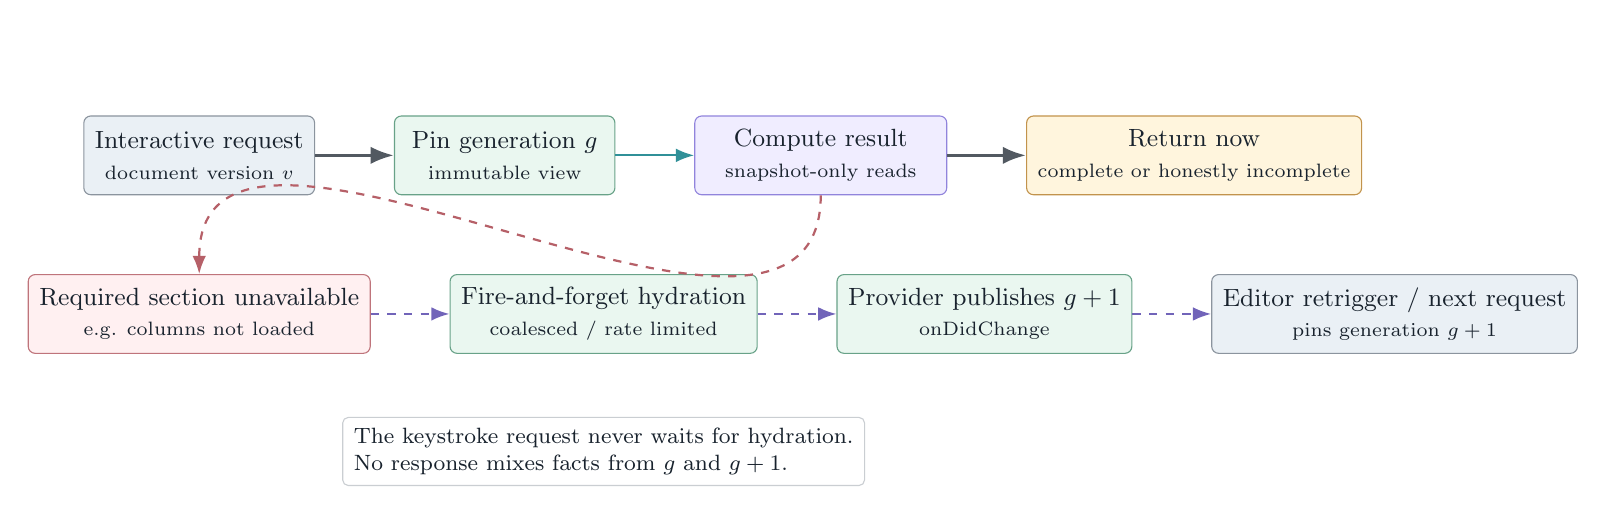
\begin{tikzpicture}[node distance=10mm and 10mm]
  \node[comp,minimum width=29mm] (req) {Interactive request\\\scriptsize document version $v$};
  \node[host,minimum width=28mm,right=of req] (pin) {Pin generation $g$\\\scriptsize immutable view};
  \node[engine,minimum width=32mm,right=of pin] (compute) {Compute result\\\scriptsize snapshot-only reads};
  \node[gate,minimum width=34mm,right=of compute] (result) {Return now\\\scriptsize complete or honestly incomplete};

  \node[risk,below=of req,minimum width=31mm] (missing) {Required section unavailable\\\scriptsize e.g. columns not loaded};
  \node[host,right=of missing,minimum width=31mm] (hydrate) {Fire-and-forget hydration\\\scriptsize coalesced / rate limited};
  \node[host,right=of hydrate,minimum width=29mm] (publish) {Provider publishes $g+1$\\\scriptsize onDidChange};
  \node[comp,right=of publish,minimum width=31mm] (retry) {Editor retrigger / next request\\\scriptsize pins generation $g+1$};

  \draw[arrow] (req)--(pin);
  \draw[dataarr] (pin)--(compute);
  \draw[arrow] (compute)--(result);
  \draw[failarr] (compute) to[out=-90,in=90] (missing);
  \draw[async] (missing)--(hydrate);
  \draw[async] (hydrate)--(publish);
  \draw[async] (publish)--(retry);

  \node[note,below=8mm of hydrate,minimum width=64mm] (noawait) {The keystroke request never waits for hydration.\\No response mixes facts from $g$ and $g+1$.};
\end{tikzpicture}}
\caption{Lazy hydration without hot-path I/O. The current request finishes from generation $g$; a later request observes $g+1$.}
\label{fig:hydration}
\end{figure}

\subsection{System and offline views}

The null provider supplies explicit offline readiness and no false catalog facts. Fixture providers simulate full, partial, and lazy-hydration states for deterministic tests. The system-catalog decorator supplies a curated names-only fallback for \code{sys} and \code{INFORMATION_SCHEMA}; live catalog facts win, identifiers are synthetic and generation-local, and the fallback does not claim column types, nullability, keys, definitions, or other facts it does not carry.

\begin{designbox}[title={No network on the feature path}]
Completion, hover, signature help, and ordinary diagnostics read the pin synchronously. A hydration request is advisory and asynchronous. Strict scripting is different by design: its host establishes an explicit freshness verdict before constructing the pinned engine. The separation makes latency and truth policy visible rather than allowing an accidental catalog call inside fuzzy matching or binding.
\end{designbox}

\section{Language feature behavior}

\subsection{Completion}

Completion first classifies cursor expectation, then uses the legacy context classifier and bound statement facts to choose producers. Producers cover statement keywords/defaults/snippets, member access, table sources, joins and foreign-key predicates, expressions and columns, variables, built-ins, star expansion, \code{INSERT}, \code{UPDATE}, \code{EXEC}, \code{DECLARE}, \code{USE}, data types, and databases.

Candidate selection is deterministic: category gates run before fuzzy matching; scores are stable; ordinal comparison breaks ties; output is capped at 600. Partial metadata does not produce an authoritative empty list. Member-access on an object with unloaded columns returns an incomplete reason and can kick background hydration.

The original differential review reproduced a statement-location fallback that bypassed comment suppression plus derived-alias, \code{UPDATE TOP}, \code{db..table}, temp-overlay, case-sensitive dedupe, and bare-\code{alias.} edit gaps. Review commit \code{b66db2d8f} repairs and regression-tests those cases. A later probe found that whitespace between a derived alias and its column list still bypassed the balance skip; commit \code{2bc5811e3} advances through trivia, captures the alias list, and applies its positional column renames in the binder. Spaced and newline-separated forms now have sketch and diagnostic-honesty coverage, and \cref{tab:fpmatrix} summarizes the full differential matrix across heads.

\subsection{Diagnostics}

Diagnostics intentionally separates two truth tiers:

\begin{itemize}
  \item \textbf{T1 lexical/structural diagnostics} come from the text, tokens, segments, and tolerant statement structure. They include unterminated strings/comments and identifiers, malformed \code{GO}, bracket/parenthesis/statement recovery, and selected syntax-error 102 cases.
  \item \textbf{T2 binder diagnostics} depend on catalog trust: invalid object 208, invalid column 207, ambiguous column 209, and routine lookup claims such as 2812 where the sketch supports them. A host freshness verdict of \code{notValidated}, partial readiness, dynamic/unsupported syntax, uncertain database context, or another recorded suppression reason prevents those warnings.
\end{itemize}

The diagnostic result records suppression counts/reasons so ``quiet because valid'' can be distinguished from ``quiet because the engine lacked authority.'' Whole-document work is resumable by statement/work unit for scheduler time slicing.

The 62-case honesty suite validates the constructs it contains, not all legal T-SQL. \Cref{sec:tiera} records newly reproduced false positives for alias assignment, cursor syntax, \code{WITHIN GROUP}, \code{AT TIME ZONE}, multi-column derived aliases, pasted NBSP, \code{UPDATE TOP}, and default-schema multipart names. These are corpus omissions and implementation defects, not evidence against the T1/T2 separation itself.

\subsection{Hover and signature help}

Hover resolves schema/database/name-chain parts, aliases, projected aliases, CTEs, derived tables, temporary/script tables, table variables, variables and parameters, catalog routines, and built-ins. H7 descriptions appear only when description readiness is true. Cross-database and \code{USE} handling share the database-context map used by binding.

Signature help scans the enclosing call without requiring a complete parse. It understands nested and grouped built-in calls, catalog functions/procedures, and \code{EXEC} argument positions. Both features stay quiet in comments, strings, SQLCMD regions, and positions where the scanner cannot make an honest call.

\subsection{Definition, folding, and symbols}

Definition has two destinations. Local aliases, variables, CTEs, temporary objects, table variables, and derived columns return in-document ranges. Catalog objects or columns route through the scripting service and return virtual content plus semantic anchors. Folding and document symbols use only the analysis snapshot and do not require catalog I/O.

\begin{table}[H]
\centering
\small
\caption{Feature truth dependencies and degradation.}
\label{tab:truth}
\begin{tabularx}{\textwidth}{@{}p{0.17\textwidth}p{0.29\textwidth}X@{}}
\toprule
\textbf{Feature} & \textbf{Primary truth input} & \textbf{When truth is incomplete}\\
\midrule
Completion & Cursor expectation, sketch, overlay, objects/columns/keys & Limit categories, return incomplete, request hydration; retain static/built-in/local candidates.\\
Diagnostics & Tokens/structure; then bound objects/columns & Preserve T1; suppress affected T2 and account for the reason.\\
Hover & Local structure or specific catalog sections & Return only facts whose section is ready; no invented type/detail.\\
Signature & Call scanner, built-ins, routine parameters & Built-ins/local syntax remain; catalog signatures require parameter readiness.\\
Definition & Local declarations or scriptable catalog target & Local range when known; virtual script with provenance; unavailable/refusal when definition truth is insufficient.\\
Folding/symbols & Snapshot, tokens, segments, sketch & Continue structurally; no metadata dependency.\\
\bottomrule
\end{tabularx}
\end{table}

\section{Scheduling, routing, and failure containment}

\subsection{Sliced diagnostics scheduler}

\path{host/scheduler.ts} is VS Code-free. A document or metadata change restarts a default 300 ms debounce. The pass then performs work in default 8 ms slices and yields by macrotask between slices. Its stamp normally combines document version and metadata generation; the scheduler rechecks the stamp before starting, after an asynchronous pass factory returns, between slices, and before publishing.

\begin{figure}[H]
\centering
\resizebox{0.97\textwidth}{!}{%
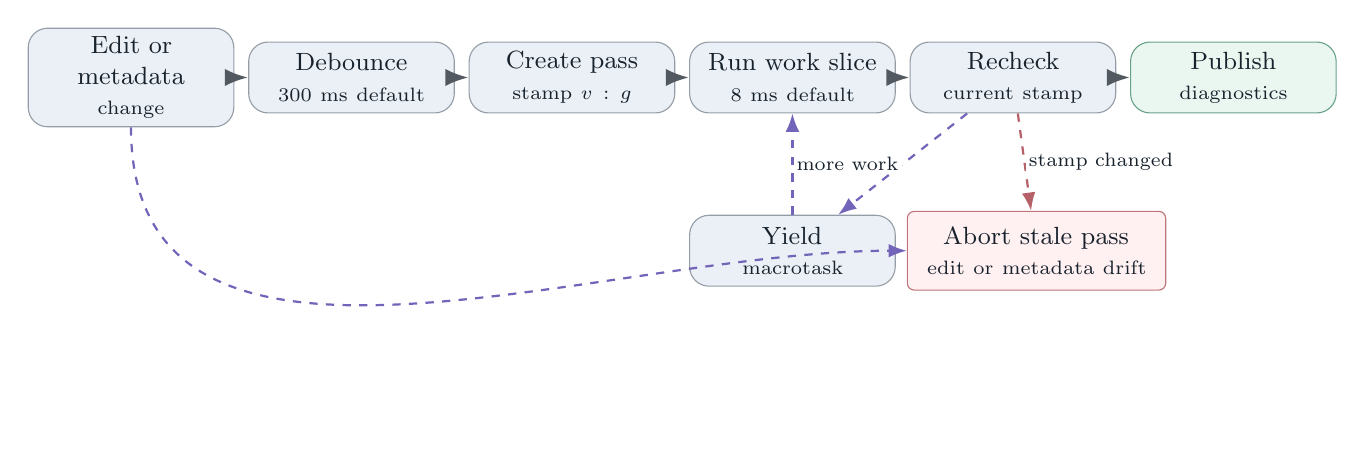
\begin{tikzpicture}[x=1cm,y=1cm]
  \node[state,text width=24mm] (change) at (0.0,2.3) {Edit or metadata\\{\scriptsize change}};
  \node[state,text width=24mm] (debounce) at (2.8,2.3) {Debounce\\{\scriptsize 300 ms default}};
  \node[state,text width=24mm] (factory) at (5.6,2.3) {Create pass\\{\scriptsize stamp $v:g$}};
  \node[state,text width=24mm] (slice) at (8.4,2.3) {Run work slice\\{\scriptsize 8 ms default}};
  \node[state,text width=24mm] (check) at (11.2,2.3) {Recheck\\{\scriptsize current stamp}};
  \node[goodstate,text width=24mm] (publish) at (14.0,2.3) {Publish\\{\scriptsize diagnostics}};

  \node[state,text width=24mm] (yield) at (8.4,0.1) {Yield\\{\scriptsize macrotask}};
  \node[risk,text width=30mm] (stale) at (11.5,0.1) {Abort stale pass\\{\scriptsize edit or metadata drift}};

  \draw[arrow] (change)--(debounce);
  \draw[arrow] (debounce)--(factory);
  \draw[arrow] (factory)--(slice);
  \draw[arrow] (slice)--(check);
  \draw[arrow] (check)--(publish);
  \draw[failarr] (check)--node[labelbox,right]{stamp changed} (stale);
  \draw[async] (check)--node[labelbox,left]{more work} (yield);
  \draw[async] (yield)--(slice);
  \draw[async] (change) to[out=-90,in=180] (stale);
\end{tikzpicture}}
\caption{Diagnostics scheduling. Old results are abandoned instead of being published after either document edits or metadata-generation drift.}
\label{fig:scheduler}
\end{figure}


\subsection{Two execution lanes}

The implementation has two materially different scheduling models. Pull features such as completion and hover execute directly in the caller's turn and are fast only because their algorithms and data access are bounded. Whole-document diagnostics can instead use a resumable pass whose work is sliced and yielded. The distinction matters because an ordinary JavaScript timeout observes control only after the event loop yields.

\begin{figure}[H]
\centering
\resizebox{0.94\textwidth}{!}{%
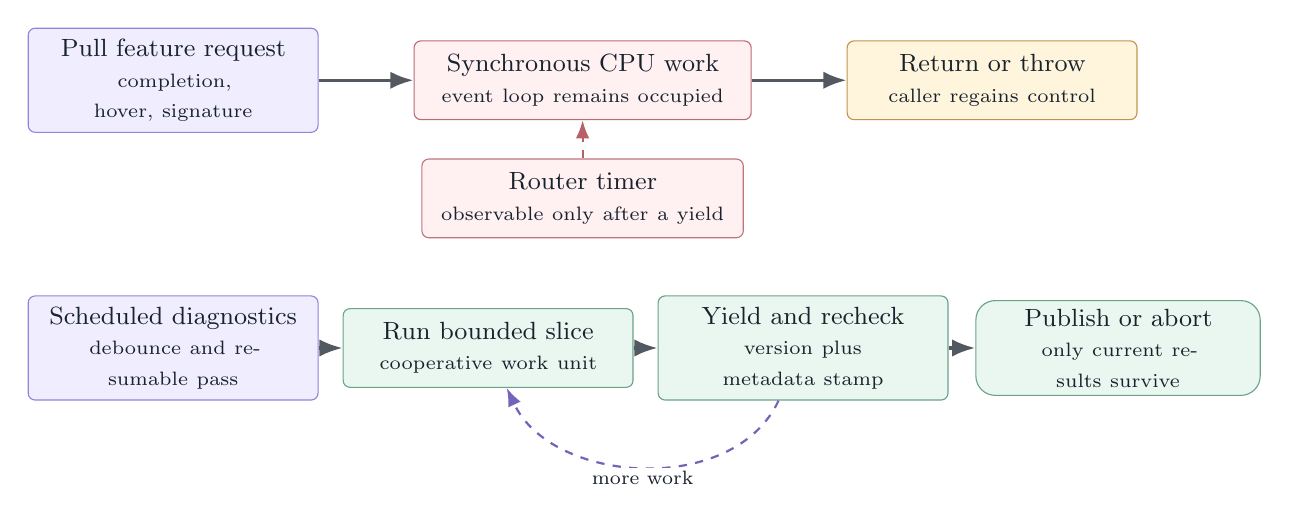
\begin{tikzpicture}[x=1cm,y=1cm]
  \node[engine,text width=34mm] (pull) at (0.0,2.4) {Pull feature request\\{\scriptsize completion, hover, signature}};
  \node[currentnode,text width=40mm] (sync) at (5.2,2.4) {Synchronous CPU work\\{\scriptsize event loop remains occupied}};
  \node[gate,text width=34mm] (pullResult) at (10.4,2.4) {Return or throw\\{\scriptsize caller regains control}};
  \node[risk,text width=38mm] (timer) at (5.2,0.9) {Router timer\\{\scriptsize observable only after a yield}};

  \node[engine,text width=34mm] (diag) at (0.0,-1.0) {Scheduled diagnostics\\{\scriptsize debounce and resumable pass}};
  \node[host,text width=34mm] (slices) at (4.0,-1.0) {Run bounded slice\\{\scriptsize cooperative work unit}};
  \node[host,text width=34mm] (yieldcheck) at (8.0,-1.0) {Yield and recheck\\{\scriptsize version plus metadata stamp}};
  \node[goodstate,text width=34mm] (diagResult) at (12.0,-1.0) {Publish or abort\\{\scriptsize only current results survive}};

  \draw[arrow] (pull)--(sync);
  \draw[arrow] (sync)--(pullResult);
  \draw[failarr] (timer)--(sync);
  \draw[arrow] (diag)--(slices);
  \draw[arrow] (slices)--(yieldcheck);
  \draw[arrow] (yieldcheck)--(diagResult);
  \draw[async] (yieldcheck) to[out=-115,in=-65] node[labelbox,below]{more work} (slices);
\end{tikzpicture}}
\caption{Execution split. Cooperative slicing bounds scheduled diagnostics; a \code{Promise.race} alone cannot interrupt synchronous extension-host work.}
\label{fig:execution-lanes}
\end{figure}

\subsection{Feature router}

\path{host/router.ts} centralizes rollout and fallback. A consumer supplies an engine preference, capability table, rollout threshold, lazy bridge factory, and optional diagnostics observer. Native work is eligible only when preference and maturity allow it. After two consecutive thrown/rejected failures for a feature, its circuit opens and later calls go directly to fallback until reset. Failures are isolated per feature, so diagnostics cannot disable completion.

The default capability table marks seven features preview, but preference still matters: under \code{sqlToolsService}, only folding and document symbols remain native because the planned bridge has no equivalent path. The bridge itself is not included in this extraction.

The router wraps native work in a default five-second \code{Promise.race}. This is a useful containment wrapper for genuinely asynchronous operations, including definition's lazy module read, but it is not CPU preemption. Completion, hover, signature, pull diagnostics, folding, and symbols compute synchronously before their already-resolved promise can race the timer. The current tests cover preference/maturity and throw-driven circuit/reset behavior; they do not demonstrate timeout interruption. Production containment therefore requires bounded algorithms, cooperative work units, or a worker boundary for any future heavy path.

\begin{figure}[H]
\centering
\resizebox{0.94\textwidth}{!}{%
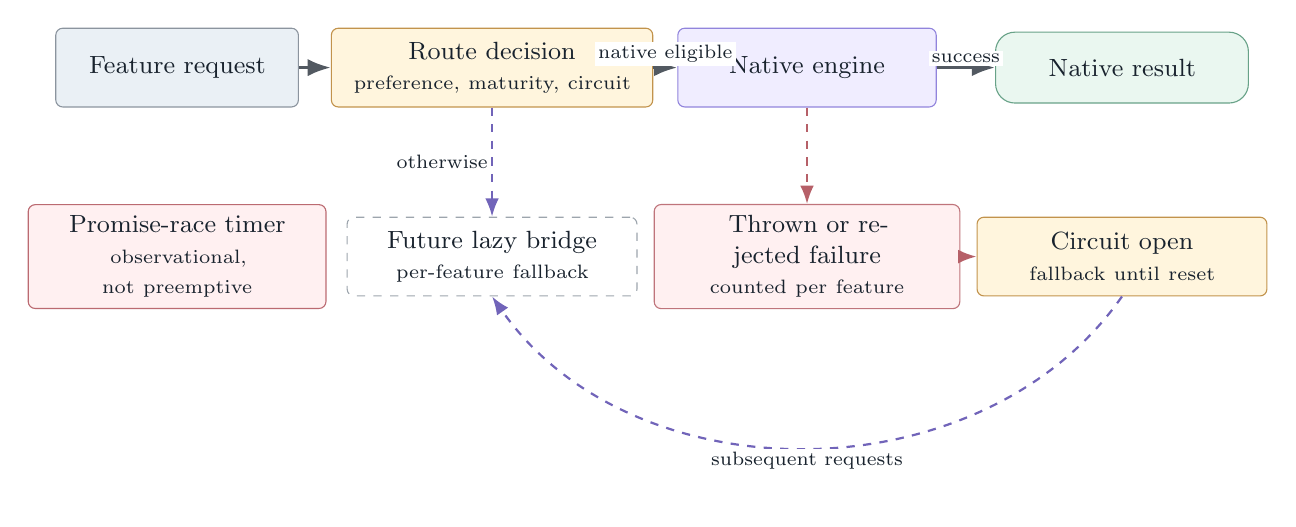
\begin{tikzpicture}[x=1cm,y=1cm]
  \node[comp,text width=28mm] (request) at (0.0,2.5) {Feature request};
  \node[gate,text width=38mm] (decision) at (4.0,2.5) {Route decision\\{\scriptsize preference, maturity, circuit}};
  \node[engine,text width=30mm] (native) at (8.0,2.5) {Native engine};
  \node[goodstate,text width=30mm] (result) at (12.0,2.5) {Native result};

  \node[currentnode,text width=35mm] (timer) at (0.0,0.1) {Promise-race timer\\{\scriptsize observational, not preemptive}};
  \node[ext,text width=34mm] (bridge) at (4.0,0.1) {Future lazy bridge\\{\scriptsize per-feature fallback}};
  \node[risk,text width=36mm] (failure) at (8.0,0.1) {Thrown or rejected failure\\{\scriptsize counted per feature}};
  \node[gate,text width=34mm] (circuit) at (12.0,0.1) {Circuit open\\{\scriptsize fallback until reset}};

  \draw[arrow] (request)--(decision);
  \draw[arrow] (decision)--node[labelbox,above]{native eligible} (native);
  \draw[arrow] (native)--node[labelbox,above]{success} (result);
  \draw[async] (decision)--node[labelbox,left]{otherwise} (bridge);
  \draw[failarr] (native.south)--(failure.north);
  \draw[failarr] (failure)--(circuit);
  \draw[async] (circuit.south) to[out=-125,in=-55] node[labelbox,below]{subsequent requests} (bridge.south);
\end{tikzpicture}}
\caption{Router containment. Maturity and per-feature circuits are implemented; the timeout is an asynchronous observation mechanism, not an interrupt for synchronous parser or binder work.}
\label{fig:router}
\end{figure}

\section{Definition and SQL scripting}

\subsection{Scripting contract}

\path{sqlScripting/api.ts} defines create, alter, create-or-alter, drop, drop-and-create, select-top, insert, update, delete, and execute operations. Results carry script text, anchors, fidelity, notes, unavailability reason, and metadata provenance.

Fidelity is explicit:

\begin{itemize}
  \item \textbf{F2} is definition-level output: a stored module definition or a table statement with the required detailed metadata.
  \item \textbf{F1} is structurally useful but incomplete output, such as a table definition degraded by missing optional details.
  \item \textbf{F0} is a template, notably DML scaffolding, and is never presented as a faithful reconstruction.
\end{itemize}

Module scripting uses token-level head rewriting so create/alter/create-or-alter changes do not replace keywords inside comments, strings, or bodies. Table scripting synthesizes columns, types, defaults/computed expressions, identity, and constraints only when corresponding metadata is ready. DML emitters produce honest templates, and degenerate shapes stay valid or explicitly editable rather than silently malformed: a target whose columns are all identity/computed emits \code{INSERT ... DEFAULT VALUES} with a fidelity note; an \code{UPDATE} with no writable non-key columns leaves an explicit \code{SET} placeholder; a missing primary key leaves an explicit \code{WHERE} placeholder. The writer records semantic anchors so definition navigation can land on the object, parameter, column, or statement rather than merely opening line zero.

\begin{table}[H]
\centering
\small
\caption{Degenerate-shape guards in the DML template emitters.}
\label{tab:dml-guards}
\begin{tabularx}{\textwidth}{@{}p{0.30\textwidth}p{0.30\textwidth}X@{}}
\toprule
\textbf{Shape} & \textbf{Emitted form} & \textbf{Why}\\
\midrule
All columns identity/computed, \code{insert} & \code{INSERT INTO [s].[t]} + \code{DEFAULT VALUES;} + note & An empty column/VALUES list is invalid T-SQL; \code{DEFAULT VALUES} inserts exactly such a row.\\
No writable non-key columns, \code{update} & \code{SET} + \code{/* add column assignments */} + note & An empty \code{SET} list is invalid; the placeholder demands an explicit user decision.\\
No primary-key metadata, keyed \code{WHERE} & \code{WHERE /* add a filter predicate */;} + note & Prevents an accidental unfiltered template while stating what is missing.\\
\bottomrule
\end{tabularx}
\end{table}

\subsection{Strict freshness flow}

The concrete scripting host calls the metadata lease's strict policy before it pins. A host-side timeout is a backstop around the metadata policy timeout. Rejection, timeout, or an unavailable strict verdict refuses the operation; explicit offline-snapshot policy can instead allow cached output with provenance and an honest banner. This makes scripting stricter than interactive completion because generated DDL is more likely to be copied and executed.


\begin{table}[H]
\centering
\small
\caption{Definition and scripting authority modes.}
\label{tab:scripting-authority}
\begin{tabularx}{\textwidth}{@{}>{\raggedright\arraybackslash}p{0.20\textwidth}>{\raggedright\arraybackslash}p{0.28\textwidth}>{\raggedright\arraybackslash}X@{}}
\toprule
\textbf{Path} & \textbf{Authority check} & \textbf{Honest outcome}\\
\midrule
Local definition & Document analysis and overlay only & Return an in-document range; no metadata lease required.\\
Catalog definition / peek & Pinned object plus lazy module-definition read & Virtual content when available; encrypted, permission, unsupported, or not-loaded reason otherwise.\\
User-facing script generation & Host resolves strict freshness, then pins & F2/F1/F0 script with provenance, or explicit refusal when strict authority is unavailable.\\
Explicit offline scripting & Host selects \code{offlineSnapshot} policy & Cached output is allowed only with source/freshness/capture provenance and an offline banner.\\
\bottomrule
\end{tabularx}
\end{table}

\begin{figure}[H]
\centering
\resizebox{0.95\textwidth}{!}{%
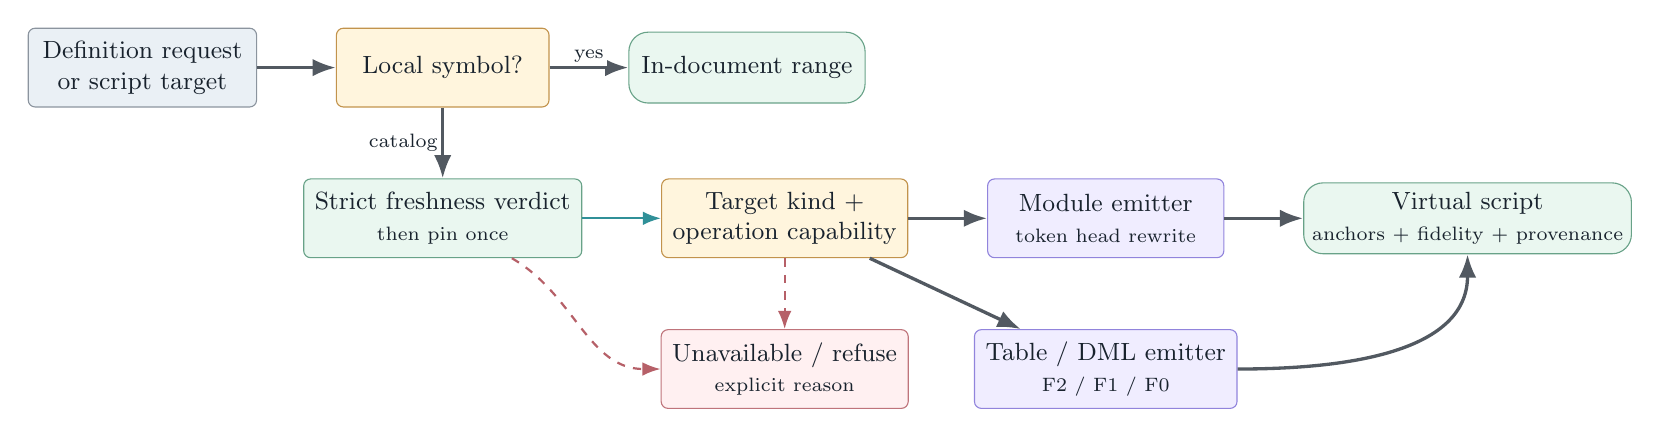
\begin{tikzpicture}[node distance=9mm and 10mm]
  \node[comp,minimum width=29mm] (target) {Definition request\\or script target};
  \node[gate,minimum width=27mm,right=of target] (local) {Local symbol?};
  \node[goodstate,minimum width=30mm,right=of local] (range) {In-document range};

  \node[host,minimum width=32mm,below=of local] (fresh) {Strict freshness verdict\\\scriptsize then pin once};
  \node[gate,minimum width=29mm,right=of fresh] (kind) {Target kind +\\operation capability};
  \node[engine,minimum width=30mm,right=of kind] (module) {Module emitter\\\scriptsize token head rewrite};
  \node[goodstate,minimum width=33mm,right=of module] (script) {Virtual script\\\scriptsize anchors + fidelity + provenance};
  \node[engine,minimum width=30mm,below=of module] (table) {Table / DML emitter\\\scriptsize F2 / F1 / F0};
  \node[risk,minimum width=30mm,below=of kind] (refuse) {Unavailable / refuse\\\scriptsize explicit reason};

  \draw[arrow] (target)--(local);
  \draw[arrow] (local)--node[labelbox,above]{yes} (range);
  \draw[arrow] (local)--node[labelbox,left]{catalog} (fresh);
  \draw[dataarr] (fresh)--(kind);
  \draw[arrow] (kind)--(module);
  \draw[arrow] (kind)--(table);
  \draw[failarr] (fresh) to[out=-30,in=180] (refuse);
  \draw[failarr] (kind)--(refuse);
  \draw[arrow] (module)--(script);
  \draw[arrow] (table) to[out=0,in=-90] (script);
\end{tikzpicture}}
\caption{Definition and scripting truth flow. Local navigation stays in the document; catalog navigation produces a provenance-bearing virtual script or an explicit refusal.}
\label{fig:scripting}
\end{figure}

\section{Observability and privacy}

The engine emits bounded spans for lexing, segmentation, parsing/sketching, completion, hover, signature help, diagnostics, definition, routing, and scripting. \path{perfTelemetry.ts} classifies \code{sqlLanguage.*} and \code{sqlScripting.*} under the existing \code{sqlLanguage} feature family; the accepted observability registry already covers those prefixes.

Normal diagnostics use safe scalar measures such as duration, counts, route, readiness, cache/hydration state, suppression reasons, and result shape. Rich completion diagnostics can classify prefix/name-part/top-label values as \code{user.text} or \code{object.name}; the shared diagnostics layer digests these by default and exposes them only under the explicitly elevated, time-bounded capture policy. The privacy claim is therefore not ``identifiers never enter an event object.'' It is that sensitive fields are classified at the call site and governed by the accepted capture/redaction boundary.

\begin{designbox}[title={Observability contract}]
Do not add raw document text, SQL batches, connection strings, result rows, or unclassified object names to a language span. New attributes must be registered and typed before emission. Performance evidence should use counts, durations, readiness and suppression state; diagnosis that truly needs content must remain an explicit elevated-capture operation.
\end{designbox}

\begin{figure}[H]
\centering
\resizebox{0.91\textwidth}{!}{%
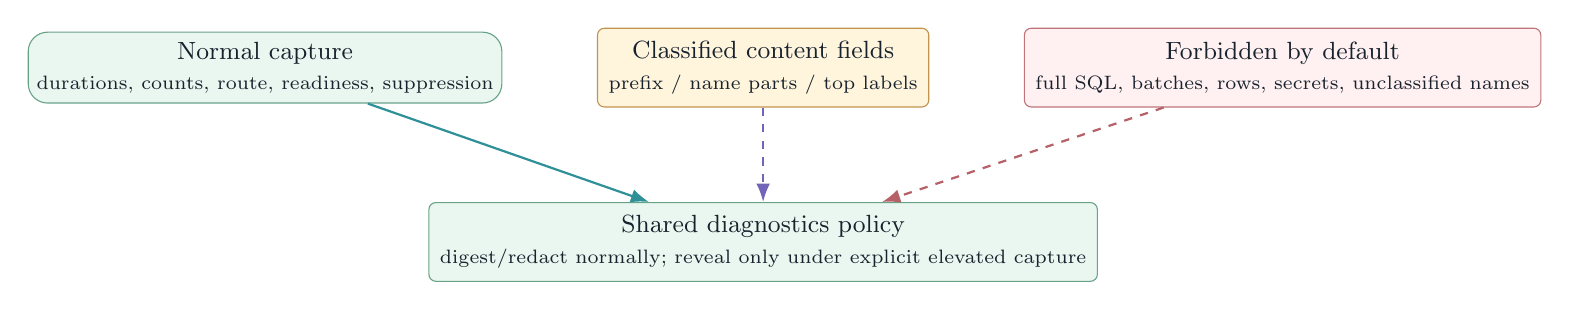
\begin{tikzpicture}[node distance=9mm and 12mm]
  \node[goodstate,minimum width=42mm] (normal) {Normal capture\\\scriptsize durations, counts, route, readiness, suppression};
  \node[gate,minimum width=42mm,right=of normal] (classified) {Classified content fields\\\scriptsize prefix / name parts / top labels};
  \node[risk,minimum width=42mm,right=of classified] (forbidden) {Forbidden by default\\\scriptsize full SQL, batches, rows, secrets, unclassified names};

  \node[host,minimum width=50mm,below=12mm of classified] (policy) {Shared diagnostics policy\\\scriptsize digest/redact normally; reveal only under explicit elevated capture};

  \draw[dataarr] (normal)--(policy);
  \draw[async] (classified)--(policy);
  \draw[failarr] (forbidden)--(policy);
\end{tikzpicture}}
\caption{Observability boundary. The implementation is privacy-classified rather than content-blind: selected identifier fields may enter spans, but the shared capture policy normally digests them and forbids unclassified SQL or secrets.}
\label{fig:observability}
\end{figure}

\section{Test design and validation}

\subsection{Focused semantic corpus}

The 15 owned language and scripting unit files execute 709 tests at the pinned head: 709 passed, zero failed, zero skipped. The value is not just volume; the suites target incomplete syntax, partial truth, deterministic ordering, stale publication, refusal behavior, and every material repair through \code{2a54ec071}. Final-head targeted validation also ran seven observability tests, for 716 passes in that selection. The preceding \code{b66db2d8f} sign-off ran 707 owned plus 47 adjacent tests (754 total); the alias-rename residual fix \code{2bc5811e3} and the degenerate-DML guard \code{2c20cc170}/\code{2a54ec071} each re-ran the full owned selection.

\begin{longtable}{@{}p{0.21\textwidth}p{0.10\textwidth}p{0.62\textwidth}@{}}
\caption{Focused language and scripting inventory.}\label{tab:tests}\\
\toprule
\textbf{Area} & \textbf{Tests} & \textbf{Principal invariants}\\
\midrule
\endfirsthead
\toprule
\textbf{Area} & \textbf{Tests} & \textbf{Principal invariants}\\
\midrule
\endhead
Completion & 82 & Member access, table sources, joins/FKs, expressions, CTE/derived/temp objects, DML/EXEC/DECLARE/USE, DDL declarations, star expansion, case-aware dedupe/edit ranges, partial-readiness honesty, latency budget, statement starts, static system catalog.\\
Cursor expectation & 17 & Category/confidence selection and quiet positions before completion producers run.\\
Core / router & 24 & Lexer coverage/Unicode whitespace, segmenter, feature routing, async timeout, maturity, fallback/circuit behavior, and LS-0 surface.\\
Definition & 56 & Aliases, variables, CTE/temp/script-local objects, catalog table/module scripts, honesty ladder, and capability routing.\\
Diagnostics & 182 & Lexical, \code{GO}, structural and recovery T1; 208/207/209 T2; expanded zero-unexpected-diagnostic honesty corpus including spaced derived aliases; overlay/case/cache suppression; lazy hydration; engine pass.\\
Diagnostics freshness & 6 & Freshness gate and scheduler drift classification.\\
Hover & 124 & Catalog and local symbol families, H7 descriptions, partial truth, \code{USE}/cross-database/MERGE, DML positions, never-hover contexts, and system catalog.\\
Journal & 3 & Normal versus elevated-capture diagnostic fields.\\
Providers & 16 & Fourslash fixture parsing, fixture behavior, real \code{CatalogBuilder}/snapshot mapping, large filtered-prefix search, and unknown-case/offline honesty.\\
Scheduler & 9 & Debounce, sliced execution, stale document cancellation, metadata drift, and asynchronous factory recheck.\\
Signature & 60 & Built-ins, nesting/grouping, catalog routines, \code{EXEC}, and honesty positions.\\
Sketch & 25 & Total structural modeling across supported statement families, multipart names, module overlays, modern expression grammar, and incomplete text.\\
System catalog & 16 & Exact TVF result shapes, static data helpers, live-over-fallback precedence, and diagnostic interaction.\\
SQL scripting & 78 & Module rewrites/anchors/honesty; table F2/F1/anchors; comment-injection safety; DML including degenerate no-writable-column shapes; capabilities/routing; provenance/offline banners.\\
Strict scripting host & 11 & Freshness policy, timeout/refusal, pin ordering, provenance, and explicit offline behavior.\\
\midrule
\textbf{Total} & \textbf{709} & \textbf{Zero failures and zero skips in the owned focused selection.}\\
\bottomrule
\end{longtable}

\subsection{Exact-head local validation and observed CI}

The full matrix was run at review commit \code{b66db2d8f}; residual commit \code{2bc5811e3} and the degenerate-DML guard \code{2c20cc170}/\code{2a54ec071} then each received exact-head validation over the full owned language/scripting selection plus observability:

\begin{table}[H]
\centering
\small
\caption{Independent local validation through final head \code{2a54ec071}; hosted lanes green at the snapshot.}
\label{tab:validation}
\begin{tabularx}{\textwidth}{@{}p{0.24\textwidth}p{0.20\textwidth}X@{}}
\toprule
\textbf{Lane} & \textbf{Result} & \textbf{Interpretation / exclusion}\\
\midrule
MSSQL build & Pass & Toolkit plus MSSQL extension typecheck, emit, extension/webview/notebook bundles.\\
MSSQL lint / repository format & Pass & Target ESLint and full-tree Prettier check completed without errors.\\
Owned language/scripting at final head & 709 pass; 0 fail & All files in \cref{tab:tests}; spaced/newline alias lists, positional renames, and degenerate DML shapes included.\\
Exact-head observability & 7 pass; 0 fail & Combined final-head targeted selection is 716/716.\\
Pre-final adjacent extended selection & 47 pass; 0 fail & Scripting service and accepted observability suites at \code{b66db2d8f}; 754 total with the then-current 707 owned tests.\\
Broad MSSQL hosted tests & 4,742 pass; 0 fail; 10 skip & Full pre-final sign-off; inverse selection excludes only two independently documented current-main Windows baseline suites: \code{Utility Tests - Path handling} and \code{QueryCompletionSoundService}.\\
SQL Projects hosted tests & 205 pass; 0 fail; 6 skip & Full pre-final sign-off in its separate VS Code host.\\
Pre-commit / diff audit & Pass & Staged hooks and \code{git diff --check} clean; validation-generated toolkit locales restored; no manifest, setting, command, or lockfile change.\\
Production online package & Pass & Released STS \code{6.0.20260827.1}; local artifact 1,542 files / 104.9 MB. Metafile contains no new language/scripting bundle input; hosted packaging and launch lanes are green at the final head.\\
\bottomrule
\end{tabularx}
\end{table}

\subsection{Review-machine scale and differential probes}

The Fable review added useful \reported{} evidence beyond the fixture suites. At pre-fix head \code{eafbbdc046}, it ran the then-current language/scripting and observability suites, hydrated the real PR04 \code{MetadataStore} with a 10,201-object B16 fixture, adapted it through \code{CatalogLanguageMetadataProvider}, and exercised \code{NativeSqlLanguageEngine}. It also ran malformed-input/depth probes and compared the curated system catalog with a live SQL Server 2025 instance. Those observations motivated the repair corpus. At \code{b66db2d8f} the original matrix was re-probed; at \code{2bc5811e3} the 12-case false-positive matrix is clean, controls still fire, completion after \code{v.} exposes renamed columns, and a table-hint control such as \code{o (NOLOCK)} remains unaffected.

\begin{table}[H]
\centering
\small
\caption{Pre-fix Fable review-machine measurements at \code{eafbbdc046}; observations, not product SLAs.}
\label{tab:reviewperf}
\begin{tabularx}{\textwidth}{@{}p{0.42\textwidth}p{0.18\textwidth}X@{}}
\toprule
\textbf{Probe} & \textbf{Observed} & \textbf{Interpretation}\\
\midrule
\code{FROM} completion, 10,201 objects & p50 4.0 ms; p95 8.7 ms & Current full-scan/sort cost is usable on the probe, but remains linear and uncached for empty-prefix catalog requests.\\
Member access / alias columns / hover & p50 about 0.1 ms; p95 $\leq$ 1 ms & Pinned lookup and local binding paths are fast in the fixture.\\
Completion at end of 2,000 statements & p50 0.8 ms; p95 35.6 ms & Tail latency shows why production size-tier budgets are still needed.\\
Diagnostics, 2,000 statements & 68.5 ms cold; near 0 cached & Analysis reuse is effective when its cache key is sound.\\
Document symbols / folding, 2,000 lines & 0.3 / 1.0 ms & Pure structural features are inexpensive on the probe.\\
Malformed/depth sweep & No throws; 5,000 parens in 13 ms & Supports total/tolerant direction; the separately found opener-at-EOF coverage hole is repaired and regression-tested.\\
\bottomrule
\end{tabularx}
\end{table}

The same live-catalog comparison found that all 157 curated built-in function names were genuine and identified two incorrect TVF result shapes. Review commit \code{b66db2d8f} removes the input handle names from \code{dm_exec_sql_text} / \code{dm_exec_query_plan}, pins their exact outputs, and adds a real \code{CatalogBuilder}/snapshot/provider-to-engine suite rather than relying only on fixture providers or hand-built handles.

The differential loop itself is worth recording because it is the reason the ordinary-SQL defects were found and proven fixed rather than argued about. Every candidate false positive was reproduced against the compiled engine before it was reported, and the identical probe inputs were re-run after each repair commit:

\begin{figure}[H]
\centering
\resizebox{0.97\textwidth}{!}{%
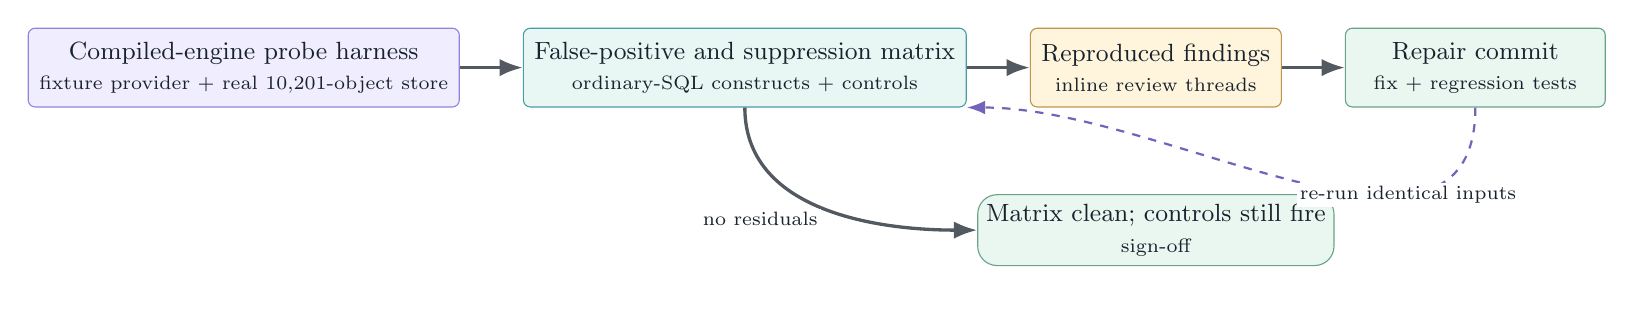
\begin{tikzpicture}[node distance=8mm and 8mm]
  \node[engine,minimum width=36mm] (harness) {Compiled-engine probe harness\\\scriptsize fixture provider + real 10,201-object store};
  \node[model,minimum width=33mm,right=of harness] (matrix) {False-positive and suppression matrix\\\scriptsize ordinary-SQL constructs + controls};
  \node[gate,minimum width=30mm,right=of matrix] (findings) {Reproduced findings\\\scriptsize inline review threads};
  \node[host,minimum width=33mm,right=of findings] (repair) {Repair commit\\\scriptsize fix + regression tests};

  \node[goodstate,minimum width=34mm,below=11mm of findings] (clean) {Matrix clean; controls still fire\\\scriptsize sign-off};
  \draw[arrow] (harness)--(matrix);
  \draw[arrow] (matrix)--(findings);
  \draw[arrow] (findings)--(repair);
  \draw[async] (repair.south) to[out=-90,in=0] node[labelbox,below right]{re-run identical inputs} (matrix.south east);
  \draw[arrow] (matrix.south) to[out=-90,in=180] node[labelbox,below left]{no residuals} (clean.west);
\end{tikzpicture}}
\caption{Differential repair loop. The same probe inputs run before and after every repair; a claim enters the review only after it reproduces, and a repair closes only after the identical matrix is clean while negative controls still fire.}
\label{fig:repair-loop}
\end{figure}

\begin{table}[H]
\centering
\small
\caption{Differential false-positive matrix across review heads. Every pre-fix cell was reproduced on the compiled engine; every final cell was re-verified with the identical input.}
\label{tab:fpmatrix}
\begin{tabularx}{\textwidth}{@{}>{\raggedright\arraybackslash}X>{\raggedright\arraybackslash}p{0.30\textwidth}>{\raggedright\arraybackslash}p{0.14\textwidth}@{}}
\toprule
\textbf{Ordinary-SQL construct} & \textbf{Pre-fix (\code{eafbbdc04})} & \textbf{Final head}\\
\midrule
\code{SELECT Total = SUM(...)} & false 207 \code{'Total'} & clean\\
\code{UPDATE ... WHERE CURRENT OF cur} & false 207 \code{'cur'} & clean\\
\code{STRING_AGG(...) WITHIN GROUP (ORDER BY ...)} & false 102 expected \code{BY} & clean\\
\code{WHERE col AT TIME ZONE 'UTC' >= ...} & false 102 twice & clean\\
\code{FROM (VALUES ...) v(a, b)} & false 208 \code{'b'} & clean\\
\code{FROM (SELECT ...) AS d (c1, c2)} (spaced) & false 208 + knock-on 207 & clean\\
\code{IS NOT DISTINCT FROM} & false 208 on the operand & clean\\
\code{label:} definition with \code{GOTO} & false 2812 at error severity & clean\\
\code{CREATE VIEW} then use across \code{GO} & false 208 on the script's own view & clean\\
NBSP pasted between name and \code{WHERE} & false 208 on a merged name & clean\\
\code{UPDATE TOP (100) target SET ...} & false 208 \code{'TOP'} & clean\\
\code{Db..Orders} default-schema shorthand & false 208 \code{'Db'} & clean\\
\midrule
Controls: unknown column / unknown object / \code{GROUP} without \code{BY} & 207 / 208 / 102 & 207 / 208 / 102\\
\bottomrule
\end{tabularx}
\end{table}

The completion-side suppression matrix followed the same discipline: trailing line comments, an opener as the document's final character, unterminated block comments, and mid-string carets all returned full candidate lists pre-fix and return zero items at the final head, while statement starts and empty documents still complete normally. The degenerate-DML probe at \code{2a54ec071} closes the loop on the scripting side (\cref{tab:dml-guards}).

\subsection{GitHub validation snapshot}

At report freeze, GitHub reports the PR open, mergeable, non-draft, labeled \code{Automated Review}, and still requiring human review. At final head \code{2bc5811e3}, action and JavaScript/TypeScript analysis, CodeQL, normalization, and CLA are green; build-and-test, package/launch, and Azure PR validation are still running. The immediately preceding head was fully green across all of those lanes and all six Linux/macOS/Windows x64/arm64 VSIX-launch jobs.

The GitHub package comparison is stronger than the absolute local size for this scope question: target and head are both 85,347 KiB for MSSQL, with zero delta for every packaged extension. Codecov reports 94.34331\% patch coverage with 1,041 changed lines uncovered and project coverage rising from 78.22\% to 79.86\%. The largest uncovered concentration is the production metadata adapter; hover, diagnostics, definition, completion, sketch/context, cursor expectation, engine, and text snapshot also retain uncovered branches.

\begin{evidencebox}
High patch coverage, 754 pre-final focused passes, and 715 final-head targeted passes support the implementation, but the important properties are semantic: one generation per answer, suppression when metadata authority is unavailable, no stale diagnostic publication, deterministic ranking, and strict scripting refusal. Coverage percentage alone cannot prove these; the differential probes were valuable precisely because they found ordinary constructs missing from the prior honesty corpus. Conversely, zero bundle-size delta proves inert packaging, not live feature quality.
\end{evidencebox}

\begin{table}[H]
\centering
\small
\caption{Largest reported pre-fix patch-coverage concentrations.}
\label{tab:coverage-hotspots}
\begin{tabularx}{\textwidth}{@{}p{0.34\textwidth}p{0.14\textwidth}p{0.16\textwidth}X@{}}
\toprule
\textbf{File / area} & \textbf{Patch coverage} & \textbf{Missing lines} & \textbf{Why it matters}\\
\midrule
\path{provider/catalogProvider.ts} & 56.79\% & 178 & The only production bridge to the merged metadata substrate; exact-head validation now adds one real builder/snapshot integration path beyond this earlier coverage report.\\
\path{features/hover.ts} & 89.09\% & 115 & Large name-chain and truth-tier surface with many context combinations.\\
\path{features/diagnostics.ts} & 94.71\% & 109 & High percentage, but uncovered branches can still be exactly the rare legal syntax that produces false squiggles.\\
\path{features/definition.ts} & 88.06\% & 97 & Crosses local-symbol resolution, scripting, async definition reads, and refusal states.\\
\path{features/completion.ts} & 92.22\% & 90 & Result edits, overlay routing, case rules, and partial-readiness paths remain semantically sensitive.\\
\path{core/text/textSnapshot.ts} & 79.03\% & 26 & Small file, but every range, anchor, and editor adaptation depends on coordinate correctness.\\
\bottomrule
\end{tabularx}
\end{table}


\section{Known limitations and review closure}


\subsection{Finding distribution}

\begin{figure}[H]
\centering
\resizebox{0.95\textwidth}{!}{%
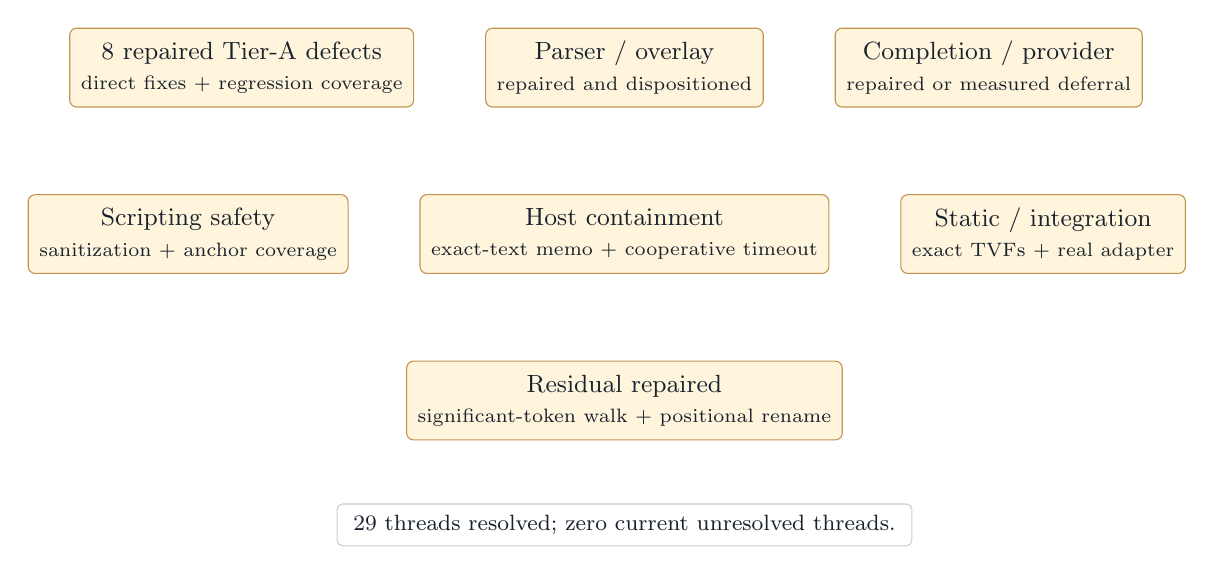
\begin{tikzpicture}[node distance=8mm and 9mm]
  \node[gate,minimum width=39mm] (tierA) {8 repaired Tier-A defects\\\scriptsize direct fixes + regression coverage};
  \node[gate,minimum width=35mm,right=of tierA] (parser) {Parser / overlay\\\scriptsize repaired and dispositioned};
  \node[gate,minimum width=35mm,right=of parser] (completion) {Completion / provider\\\scriptsize repaired or measured deferral};

  \node[gate,minimum width=35mm,below=11mm of parser] (host) {Host containment\\\scriptsize exact-text memo + cooperative timeout};
  \node[gate,minimum width=35mm,left=of host] (script) {Scripting safety\\\scriptsize sanitization + anchor coverage};
  \node[gate,minimum width=35mm,right=of host] (data) {Static / integration\\\scriptsize exact TVFs + real adapter};
  \node[gate,minimum width=35mm,below=11mm of host] (copilot) {Residual repaired\\\scriptsize significant-token walk + positional rename};

  \node[note,below=8mm of copilot,minimum width=73mm] (total) {29 threads resolved; zero current unresolved threads.};
\end{tikzpicture}}
\caption{Review disposition map at final head \code{2a54ec071}. All current threads have explicit dispositions.}
\label{fig:findings-map}
\end{figure}

\subsection{Review snapshot: 29 dispositioned threads}

The pre-fix PR had 26 current review threads at \code{eafbbdc046}: two from Copilot and 24 from a later source-attributed Fable review posted through the PR author's account. Every initial thread received an explicit disposition and was resolved after review commit \code{b66db2d8f}. One immediate Copilot follow-up about the documented newline precondition of \code{withHeader} was dispositioned after a complete production call-site audit. A later Fable probe then found one valid residual variant: whitespace between a derived alias and its column list prevented the raw-token-index guard from seeing the opening parenthesis. Commit \code{2bc5811e3} fixes that variant, adds full positional alias semantics, and closes the 28th thread. A final Copilot thread then flagged that all-identity/computed targets produced invalid empty \code{INSERT}/\code{SET} lists from the DML templates; that reproduced exactly as reported, and commits \code{2c20cc170}/\code{2a54ec071} close the 29th thread with the \cref{tab:dml-guards} guards and a regression test. At report freeze the live API returns zero unresolved threads.

The two original Copilot threads were narrow and are fixed:

\begin{enumerate}
  \item \path{sqlScripting/scriptWriter.ts} now counts standalone CR, LF, and CRLF correctly in writer and prepended-header anchors, with mixed-ending regression coverage.
  \item \path{sqlScripting/scriptingService.ts} now says synonym definition text is unavailable through this scripting engine rather than making an inaccurate hydration claim.
\end{enumerate}

\subsection{Tier A: ordinary-SQL trust defects}\label{sec:tiera}

The eight original Tier-A findings were not architectural failures, but they were the exact user-trust failure class the diagnostic honesty design is intended to prevent. All eight have direct repairs; commit \code{2bc5811e3} closes the last formatting variant of the fifth repair, and the final scripting-guard round closes the remaining Copilot thread.

\begin{enumerate}[label=\textbf{A\arabic*.},leftmargin=2.2em,itemsep=5pt]
  \item \textbf{Trailing comments and unterminated constructs} (\path{nativeEngine.ts}). Lexical suppression now runs before the undefined-statement fallback; comment, string, SQLCMD, and exact-EOF opener cases return no completion.
  \item \textbf{Alias assignment and positioned update} (\path{diagnostics.ts}). Select-list \code{alias = expr} heads and \code{CURRENT OF} cursor names are excluded from column diagnostics.
  \item \textbf{\code{WITHIN GROUP (ORDER BY ...)}} (diagnostics / keyword data). Contextual \code{WITHIN} plus ordered-set clause handling prevents the false missing-\code{BY} recovery.
  \item \textbf{\code{AT TIME ZONE}} (diagnostics / keyword data). Contextual \code{AT}/\code{ZONE} entries break the false expression-unit run without reserving legal identifiers.
  \item \textbf{Derived/VALUES alias lists} (\path{sketch/index.ts}, \path{binder.ts}). The parser advances through trivia, captures the balanced alias list, and the binder applies names positionally. Unspaced, spaced, and newline-separated lists cannot create phantom sources; VALUES columns gain their declared names and renamed-away originals no longer resolve.
  \item \textbf{Non-breaking space in pasted SQL} (\path{lexer.ts}). Unicode horizontal space separators, including U+00A0, are whitespace rather than identifier characters.
  \item \textbf{\code{UPDATE TOP (n) target}} (\path{sketch/index.ts}). Update sketching skips TOP count forms and optional PERCENT before reading the target.
  \item \textbf{Default-schema shorthand \code{db..table}} (\path{sketch/index.ts}). Empty multipart components are preserved, and binder arity uses raw parts to reach honest cross-database/linked-server handling.
\end{enumerate}

\subsection{Tier B/C: correctness, safety, and evidence hardening}

The other 16 Fable threads were triaged in five groups. Material correctness and safety issues were fixed; two design/optimization suggestions received narrower evidence-backed dispositions:

\begin{table}[H]
\centering
\small
\caption{Source-attributed review findings and final dispositions.}
\label{tab:tierbc}
\begin{tabularx}{\textwidth}{@{}p{0.20\textwidth}p{0.48\textwidth}X@{}}
\toprule
\textbf{Group} & \textbf{Findings} & \textbf{Disposition}\\
\midrule
Parser / overlay honesty & \code{IS NOT DISTINCT FROM}; labels/synonyms; script-created modules and qualified objects; EOF coverage; GO corpus. & Repaired with grammar, overlay, lexical-coverage, and table-driven regression tests.\\
Completion / provider & Temp DML targets; case-aware dedupe; bare-\code{alias.} edits; filtered prefix cap; unknown case rule; empty-prefix scan. & Correctness paths repaired. Prefix search grows past 1,200 filtered-out items. Empty-prefix caching is deferred: measured p95 is 8.7 ms and cache invalidation complexity is not justified without a budget regression.\\
Host correctness & Same-version/same-length cache collision; synchronous router timeout semantics. & Analysis and diagnostic memos require exact text. Async timeout is tested and cooperative semantics documented; synchronous interactive work remains self-bounding and diagnostic publication remains sliced.\\
Scripting safety & Comment placeholders/refusals can interpolate pathological identifiers or type text; all-identity/computed targets emitted invalid empty \code{INSERT}/\code{SET} lists. & Reused \code{sanitizeCommentText} across DML and refusal paths; degenerate shapes now emit \code{DEFAULT VALUES} or explicit placeholders (\cref{tab:dml-guards}); adversarial and degenerate-shape tests pass.\\
Static data / integration evidence & Two \code{dm_exec_*} TVF result schemas; fixture-only production adapter coverage. & Corrected exact TVF shapes and added real builder/snapshot/provider-to-engine coverage.\\
\bottomrule
\end{tabularx}
\end{table}

All current findings are resolved or explicitly dispositioned in the PR. The final-head targeted matrix pins the spaced-alias-list reproduction, its rename semantics, and the degenerate-DML guards. The preceding fully green broad matrix plus final targeted evidence prove regression stability against the encoded corpus; neither is a claim of complete T-SQL equivalence.

\subsection{Deliberate implementation limits}

\begin{itemize}
  \item The sketch is not a full T-SQL AST and the feature set is not a ScriptDOM equivalence claim.
  \item Highlights and semantic tokens are off.
  \item The bridge/fallback adapter is a router seam, not an implementation in this PR.
  \item The metadata adapter's lazy kick currently refreshes the full metadata ladder; section-specific hydration remains a future optimization.
  \item The system fallback is names-only and deliberately cannot support type/detail/key/definition claims.
  \item No live editor consumer, settings hierarchy, provider registration, Query Studio integration, AI completion, SQL document service, sqlcmd preprocessing, execution batch splitter, or query execution helper ships here.
  \item Unit fixtures cover a wide semantic corpus and the review added one SQL Server 2025/static-data plus 10,201-object store probe, but broad real-server collation, permissions, dynamic SQL, uncommon grammar, Azure/serverless behavior, and remote extension-host performance remain preview validation work.
\end{itemize}

\subsection{Branch-drift boundary}

The topic includes extraction base \code{95cf790e5}; the live PR API identifies base \code{53b707bbe}; and current repository \code{main} is \code{c6d2baa442}. The exact topic is four commits ahead of and nine commits behind current \code{main}. The mainline-only commits touch controller, document-service, package, test, and extension infrastructure. The PR remains mergeable while the final hosted rerun completes; every subsequent consumer must nevertheless start from refreshed \code{main} and repeat build, focused/broad semantics, package, launch, and review checks.

\section{Integration and graduation plan}

\subsection{Next implementation step}

The next PR should be a gated consumer, not another implicit activation edit scattered across the extension. The source-only trust findings in \cref{sec:tiera} are closed; the consumer PR should then:

\begin{enumerate}
  \item add one composition root that adapts VS Code documents and result types to the consumer-neutral contracts;
  \item require \code{mssql.enableExperimentalFeatures} and a dedicated default-off native-language/AI feature flag before registration;
  \item hide contributed commands and UI with complete manifest \code{when} clauses, not only disabled command enablement;
  \item choose native versus existing behavior through the router, provide the real lazy bridge, and preserve per-feature fallback;
  \item wire the metadata provider from the accepted shared catalog service and dispose leases/change subscriptions correctly;
  \item carry perftest and scenario tests for activation-off invisibility, gated activation, latency, fallback, and stale-result suppression; and
  \item avoid coupling AI completion to a global language-provider cutover--AI can be an early gated consumer of the same analysis/provider seam.
\end{enumerate}

\subsection{Graduation gates}

Before moving from private preview toward default-on, validation should add:

\begin{enumerate}
  \item a live-SQL truth corpus across supported versions, Azure variants, collations, permissions, synonyms, temporary/script objects, and cross-database contexts;
  \item side-by-side native/STS result comparison with categorized differences rather than raw count parity;
  \item interactive p50/p95/p99 budgets for completion/hover/signature and sliced whole-document diagnostics across document/catalog size tiers;
  \item remote and web/virtualized extension-host CPU/memory measurements plus metadata hydration/retrigger behavior;
  \item UI-level tests for flag hierarchy, command/menu invisibility, reload semantics, circuit-breaker fallback, and disabling the preview; and
  \item an explicit privacy audit of elevated rich fields, journal/export behavior, and any AI consumer payload boundary.
\end{enumerate}


\begin{table}[H]
\centering
\small
\caption{Minimum gates before the first user-reachable preview consumer.}
\label{tab:activation-gates}
\begin{tabularx}{\textwidth}{@{}p{0.31\textwidth}p{0.16\textwidth}X@{}}
\toprule
\textbf{Gate} & \textbf{Current state} & \textbf{Required closure}\\
\midrule
Ordinary-SQL trust corpus & Current review closed & Original eight cases plus spaced/newline alias-list variants and positional renames are repaired; continue expanding the live differential corpus.\\
Production metadata adapter & Partial & One real \code{CatalogBuilder}/snapshot/provider/engine path now exists; extend it with generation drift, partial readiness, and live-server variants.\\
Router and long-work containment & Partial & Explicit synchronous limitation, bounded algorithms, timeout test for yielding paths, and cooperative/worker plan for heavy work.\\
Private-preview composition & Not present & One default-off composition root with hierarchical flags, complete manifest visibility gates, disposal, and disable/reload tests.\\
Bridge/fallback & Interface only & Concrete lazy bridge, provider ownership, telemetry, and fallback behavior under throw/timeout/circuit.\\
Latency and memory & Probe only & p50/p95/p99 by document/catalog tier on local and remote extension hosts.\\
Privacy & Architecture present & Elevated-capture audit and product-level journal/export test once a consumer exists.\\
\bottomrule
\end{tabularx}
\end{table}

\begin{table}[H]
\centering
\small
\caption{Mechanism-to-evidence traceability.}
\label{tab:trace}
\begin{tabularx}{\textwidth}{@{}p{0.25\textwidth}p{0.31\textwidth}X@{}}
\toprule
\textbf{Mechanism} & \textbf{Current evidence} & \textbf{Next proof}\\
\midrule
Pure analysis contracts & Import shape, fixture engines, hosted unit tests & Consumer adapter tests in the first activation PR.\\
Pinned-generation metadata & Provider types and fixture/null/system tests; reviewer real-store probe & CI end-to-end real-snapshot suite plus forced generation change.\\
No hot-path network wait & Synchronous pin contract, lazy kick tests, and reviewer real-store timings & Instrumented product/perftest assertion under hydration.\\
Completion determinism & Category/rank/ordinal tests; repaired suppression, dedupe, overlay, edit-range, and derived-alias cases & Add cross-platform replay and product-level latency budgets.\\
Diagnostic honesty & T1/T2 split, expanded honesty suite, freshness/drift tests, Tier-A repairs, and spaced-alias regression & Add a real-server/native-vs-STS differential corpus.\\
Stale-result suppression & Deterministic scheduler stamp tests & VS Code integration under edit/hydration storms.\\
Strict scripting provenance & Freshness/refusal/offline and emitter tests & Live permissions/encryption/definition corpus.\\
Failure containment & Three preference/maturity/throw-circuit/reset tests; sliced scheduler tests & Cooperative bound for synchronous work, timeout test, real bridge/fallback telemetry.\\
Private-preview invisibility & No manifest/controller/bundle inputs; zero package delta & Manifest/runtime gate tests when activation is introduced.\\
\bottomrule
\end{tabularx}
\end{table}

\section{Final assessment}

\begin{takeawaybox}
PR \#22860 is a strong extraction boundary. It converts the earlier language-service plan into a concrete, testable library without prematurely changing product behavior. The core architecture is the right one: tolerant analysis over unfinished text; a claim hierarchy that preserves lower-level truth; one pinned metadata generation per answer; explicit readiness and suppression; deterministic candidate order; sliced, stale-safe diagnostic publication; provenance-bearing scripting; and per-feature rollout/fallback.

The later review materially strengthened the correctness disposition. The eight original ordinary-SQL trust defects, the spaced/newline alias-list variant, and the degenerate-DML template shapes now have direct repairs and regression cases; the broader cache-identity, completion-edit, provider, scripting-sanitization, static-data, and real-adapter gaps are closed or explicitly dispositioned. The alias capture also implements the actual positional rename semantics instead of merely skipping commas, and the DML emitters now refuse to produce syntactically invalid degenerate templates. The router timeout is accurately documented as cooperative rather than preemptive for synchronous work. The broad matrix, the final targeted matrix, and every reported hosted lane are green at the snapshot. Zero package delta proves current users cannot reach the code, not full language equivalence.
\end{takeawaybox}

\begin{statusbox}[title={Decision statement}]
Recommended disposition at this snapshot: \textbf{automated source review is complete for the inert foundation at \code{2a54ec071}}. All 29 threads have explicit dispositions, the live API reports zero unresolved threads, the exact-head targeted matrix is green, every reported hosted lane is green, and the PR is mergeable. Human review of the small post-sign-off fix delta (\code{b66db2d8f..2a54ec071}) is the remaining merge gate. A later consumer PR must independently satisfy the full private-preview umbrella/feature gates, invisible command/menu contribution, runtime fail-closed behavior, and integration-level scenario validation before exposing the engine through Query Studio, a VS Code provider, command, or AI context path.
\end{statusbox}

\section*{Evidence and source map}
\addcontentsline{toc}{section}{Evidence and source map}

\begin{statusbox}[title={Reproducibility note}]
This report is pinned to an active PR. Review threads, Actions conclusions, main-branch refs, coverage, and mergeability are observations at the stated snapshot. Re-fetch the head and live PR state after any code or base-branch change before reusing its final disposition.
\end{statusbox}

\small
\begin{longtable}{@{}>{\raggedright\arraybackslash}p{0.23\textwidth}>{\raggedright\arraybackslash}p{0.70\textwidth}@{}}
\toprule
\textbf{Evidence class} & \textbf{Primary sources used}\\
\midrule
PR state & \href{https://github.com/microsoft/vscode-mssql/pull/22860}{PR \#22860}, head \code{2a54ec071}, extraction base \code{95cf790e5}, live API base \code{53b707bbe}, 29 dispositioned threads / zero unresolved, Copilot review, source-attributed Fable reviews and probe reports, the sign-off comment, final-head targeted validation, hosted lane state, package-size bot, and Codecov report.\\
Public API / host & \path{extensions/mssql/src/sqlLanguage/api.ts}; \path{host/nativeEngine.ts}; \path{host/router.ts}; \path{host/scheduler.ts}; \path{host/scriptingHost.ts}.\\
Analysis core & \path{core/text/textSnapshot.ts}; \path{core/lexer.ts}; \path{core/segmenter.ts}; \path{core/sketch/*}; \path{core/parser/cursorExpectation.ts}; \path{core/binder.ts}; \path{core/overlay.ts}; database/name/fuzzy/quote helpers.\\
Language features & \path{features/completion.ts}; \path{diagnostics.ts}; \path{hover.ts}; \path{signatureHelp.ts}; \path{definition.ts}; \path{folding.ts}; \path{documentSymbols.ts}; generated keyword/built-in/default/system data.\\
Metadata seam & \path{provider/types.ts}; \path{catalogProvider.ts}; \path{systemCatalogView.ts}; \path{nullProvider.ts}; \path{fixtureProvider.ts}; merged metadata-service implementation from PR \#22836.\\
SQL scripting & \path{extensions/mssql/src/sqlScripting/api.ts}; \path{scriptingService.ts}; \path{scriptWriter.ts}; module/table/DML emitters; strict host under \path{sqlLanguage/host}.\\
Observability & \path{extensions/mssql/src/perf/perfTelemetry.ts}; accepted diagnostics registry and privacy contracts already in \code{main}; journal tests.\\
Tests & Fifteen \path{extensions/mssql/test/unit/sqlLanguage*.test.ts} and \path{sqlScripting*.test.ts} files; hosted JUnit XML; independent build/lint/broad-suite/package record summarized in \cref{tab:validation}.\\
Design intent & \path{vscode-ext-refactor/language-service-docs/05-tsql-language-service-design.md}; \path{current_completions_parser_design.md}; \path{PROGRESS.md}; proposed diagnostics/completion designs. Code controls where historical/future design differs from the extraction.\\
Private-preview policy & Accepted PR04 preview-gating implementation plus the current PR manifest and activation diff; PR05 adds no consumer registration, setting, or command.\\
\bottomrule
\end{longtable}

\end{document}
